\documentclass[11pt]{article}

\usepackage[letterpaper, margin=0.7in]{geometry}
\usepackage{graphicx}
\usepackage{subcaption}
\usepackage{cleveref}
\usepackage{listings}
\usepackage{multicol}
\usepackage{tikz}
\usepackage{bm}
\usepackage{minted}
\usetikzlibrary{arrows}
\usepackage{wrapfig}
\usepackage{amsmath}
\usepackage{amssymb}
\usepackage[section]{placeins}
\usepackage{pgfplots,wrapfig}  
\pgfplotsset{compat=newest} 
\pgfplotsset{plot coordinates/math parser=false} 
\newlength\figureheight 
\newlength\figurewidth 
\setlength{\parindent}{0pt}

\begin{document}

\begin{center}

COMP6212 Assignment 1 : Shakib-Bin Hamid 25250094 sh3g12

\end{center}

\section{Efficient Frontier}

Let a portfolio of $N$ assets be $\bm{\pi}$, whose expected return is $\bm{\mu}$ and the 
co-variance is $\bm{\Sigma}$. \\

\subsection{Efficient Frontier with 3 Assets}

\begin{wrapfigure}{!h}{0.45\textwidth}
	\vspace{-2cm}
  \begin{center}
    \resizebox {0.4\textwidth} {!} {% This file was created by matlab2tikz.
%
%The latest updates can be retrieved from
%  http://www.mathworks.com/matlabcentral/fileexchange/22022-matlab2tikz-matlab2tikz
%where you can also make suggestions and rate matlab2tikz.
%
\begin{tikzpicture}

\begin{axis}[%
width=4.521in,
height=3.455in,
at={(0.758in,0.551in)},
scale only axis,
xmin=0.02,
xmax=0.2,
xlabel style={font=\color{white!15!black}},
xlabel={\Large{Risk (V)}},
ymin=0.11,
ymax=0.2,
ylabel style={font=\color{white!15!black}},
ylabel={\Large{Expected Return (E)}},
axis background/.style={fill=white},
title style={font=\bfseries},
title={\Large{Efficient Portfolio Frontier}},
xmajorgrids,
ymajorgrids,
legend style={at={(0.646,0.213)}, anchor=south west, legend cell align=left, align=left, draw=white!15!black}
]
\addplot [color=red, line width=3.0pt]
  table[row sep=crcr]{%
0.0392232270276368	0.123076923076923\\
0.0445134244448113	0.131623931623932\\
0.0558620045678976	0.14017094017094\\
0.0700946304111869	0.148717948717949\\
0.0857876793614043	0.157264957264957\\
0.102271059970778	0.165811965811966\\
0.119217400342715	0.174358974358974\\
0.138250340140825	0.182905982905983\\
0.166128871535853	0.191452991452991\\
0.2	0.2\\
};
\addlegendentry{Frontier}

\addplot [color=blue, draw=none, mark size=1.3pt, mark=*, mark options={solid, blue}]
  table[row sep=crcr]{%
0.080495429441755	0.152464631405146\\
0.0586842877403314	0.141449498010093\\
0.097843171452764	0.157526651003101\\
0.0843279566532557	0.130715741868899\\
0.0690982627609729	0.139482199761925\\
0.106451639188587	0.159459177112842\\
0.0791290887018972	0.153474335086426\\
0.117146861548647	0.172360961018159\\
0.0787590662249076	0.1518123668259\\
0.095590667259509	0.160798781088421\\
0.0722532075283603	0.116781042251636\\
0.130342280965643	0.152635625071473\\
0.0835464974184604	0.140374611684177\\
0.118085453403673	0.173650119962316\\
0.0754854369198997	0.150849258835949\\
0.0793827986282716	0.148603426326158\\
0.0750987838545445	0.151302294720501\\
0.0720408029394771	0.14917842697788\\
0.107988655377768	0.16202729697618\\
0.0934321480945381	0.160651996165468\\
0.0661384524789506	0.133595661049102\\
0.0830717964004759	0.153762379514578\\
0.0512538718137417	0.125537392937739\\
0.117904929312031	0.171560284151031\\
0.0822798850641827	0.135638178937451\\
0.0655975088348891	0.140385128825852\\
0.0656080282085027	0.145046616324208\\
0.065826415890757	0.143754133249167\\
0.0723403014552528	0.133895927845577\\
0.0666559604617539	0.139033960136715\\
0.124378785464722	0.148342105217536\\
0.0842085168753325	0.154200661603322\\
0.0681789785878722	0.145265619005709\\
0.099791985935791	0.143238181930397\\
0.0946821808985729	0.160807577183566\\
0.0770923731010945	0.138841229662731\\
0.0753872318657339	0.151560910256801\\
0.117370379839209	0.155919230218454\\
0.115011301281024	0.172203176276271\\
0.0708292609778084	0.119744029743706\\
0.174328939116651	0.189846123956729\\
0.0781182327995599	0.150861323324786\\
0.112976072960543	0.171190129611143\\
0.0768103196509027	0.141395137792615\\
0.0851638614793953	0.156931446507568\\
0.11683933147533	0.173129129887712\\
0.0930686505346942	0.136920359880709\\
0.0685748603234679	0.140879681607451\\
0.068964573628841	0.127299325406174\\
0.0887789016325956	0.155536472150768\\
0.108617509966948	0.136579930477388\\
0.0593887730579937	0.138209201186662\\
0.107238182280698	0.167496186218074\\
0.124155033874371	0.176110389616136\\
0.096333155214537	0.160930471010794\\
0.111817142536496	0.16995108580561\\
0.0670559875105171	0.120369741030219\\
0.124088584602731	0.169669388079225\\
0.118891514129702	0.157314013523634\\
0.0693831588114307	0.147706053676244\\
0.0818573424573268	0.142106910138418\\
0.123082407021245	0.173498907916256\\
0.0910042901198481	0.15724594293039\\
0.118144541002869	0.173744502464097\\
0.0733596086524069	0.148140361458725\\
0.0889700167552594	0.157625024720334\\
0.073253542792152	0.149494937052732\\
0.0959498351568133	0.162564341216811\\
0.0991553494532118	0.163581802795384\\
0.0787677314364844	0.152054887877629\\
0.0907613899858104	0.154771042719299\\
0.12568685355509	0.174174518406362\\
0.0733630527162351	0.145577906988818\\
0.0923484916104742	0.146269972346275\\
0.0975420964073408	0.141927419054204\\
0.045591269865269	0.132321202861959\\
0.0914093135238453	0.155970415503178\\
0.096484519607753	0.16080497656299\\
0.0815381866528432	0.141795967475022\\
0.0852349038672028	0.154212830821872\\
0.112831778740422	0.157700804551902\\
0.123808532831889	0.176641525960269\\
0.0789337302107972	0.153446598934787\\
0.0964998420056591	0.162806132873303\\
0.0728084617243153	0.138340249531696\\
0.0754292678303717	0.151621095575614\\
0.12930957220291	0.17227118422087\\
0.075546729503246	0.150541863869806\\
0.099292200671396	0.161722191158609\\
0.0840291687866919	0.132335877064247\\
0.114124098658465	0.171797978589674\\
0.0770992357644214	0.148665143154413\\
0.0692655203787419	0.135529931191994\\
0.121383495830995	0.14139939457319\\
0.0861661460332523	0.149466741434447\\
0.0810971286328018	0.150186867113442\\
0.0598813261523254	0.142691744118496\\
0.143411178105358	0.177987611166573\\
0.0983225734267333	0.140162773114559\\
0.0657733578906526	0.143699798597633\\
};
\addlegendentry{Portfolio}

\end{axis}
\end{tikzpicture}% }
	\caption{Efficient Portfolio}
	\label{fig:q1-a-efficient-portfolio}
  \end{center}
	\vspace{-1cm}
\end{wrapfigure}

According to the paper, the expected return of the portfolio, 
$E = \sum_{i=1}^N\pi_i\mu_i = \bm{\pi}^t\bm{\mu}$. The risk is analogous to the variance of
the returns, i.e. $V = \sum_{i=1}^N\sum_{j=1}^N\sigma_{ij}\pi_i\pi_j = \bm{\pi}^t\bm{\Sigma}\bm{\pi}$.\\

Given $\bm{\mu} = \bm{m}$ and $\bm{\Sigma} = \bm{C}$ for a $3$ assets, we can generate 100 random
portfolios, where each portfolio $\bm{\pi} = (\pi_1 \pi_2 \pi_3)^t$ s.t. $\bm{1}^t\bm{\pi} = 1$ by
\mintinline{matlab}|y=randn(3,1); y=y/norm(y,1)|. Then we can calculate $E-V$ for each of the portfolios by
\mintinline{matlab}|E=y'*m; V=sqrt(y'*C*y)|.\\

Finally I make the scatter plot and on the same figure I plot the efficient frontier using
\mintinline{matlab}|estimateFrontier| function. As expected all the random portfolios were on the
correct one side of the frontier. 

\subsection{Efficient Frontier with 2 Assets}

To prepare three 2 asset porfolios, we remove the data points that are not necessary, i.e. that has
the third asset. First I plotted random returns generated by the 2 asset mean and variance using
\mintinline{matlab}|mvnrnd|. As can be noticed from Figure \ref{fig:q1-b-return-distribution}, asset
2 and 3 are almost uncorrelated, asset 1 and 2 are negatively correlated, asset 1 and 3 are positively
correlated.\\

\begin{figure}[!h]
	\vspace{-0.5cm}
	\centering 
	\resizebox {0.7\textwidth} {!} {% This file was created by matlab2tikz.
%
%The latest updates can be retrieved from
%  http://www.mathworks.com/matlabcentral/fileexchange/22022-matlab2tikz-matlab2tikz
%where you can also make suggestions and rate matlab2tikz.
%
\definecolor{mycolor1}{rgb}{0.00000,0.70000,0.20000}%
%
\begin{tikzpicture}

\begin{axis}[%
width=4.255in,
height=4.255in,
at={(2.592in,0.978in)},
scale only axis,
xmin=-1,
xmax=1,
xlabel style={font=\color{white!15!black}},
xlabel={\Huge{Asset 1 Return}},
ymin=-1,
ymax=1,
ylabel style={font=\color{white!15!black}},
ylabel={\Huge{Asset 2 Return}},
axis background/.style={fill=white},
title style={font=\bfseries},
title={\huge{Portfolio 1 Return Distribution}},
xmajorgrids,
ymajorgrids
]
\addplot [color=red, draw=none, mark=*, mark options={solid, red}, forget plot]
  table[row sep=crcr]{%
0.174151002623628	0.00902610724528322\\
0.202284403398903	0.0129408719558233\\
0.00488963473203964	0.435227800633213\\
0.106141547394353	0.131740753651927\\
0.134870665435126	-0.0938460871794249\\
0.0682898058865507	0.195106877869821\\
-0.0573633587199946	0.758880039316307\\
0.0343848145740485	0.205645075821813\\
0.208313565386524	-0.116444607734168\\
-0.0520430806683847	0.264047146988072\\
-0.0297012094313748	0.443664615574465\\
0.127930775580846	0.0417889571431549\\
0.103183587467997	0.219723805681077\\
0.0996384996837877	0.225586137936828\\
0.068111673287765	0.25194814903904\\
0.121195707974088	0.237808758850137\\
0.163960572387273	0.0724733984381672\\
0.0530533225144975	0.32042898645123\\
0.208407579421589	-0.11794240288881\\
0.0805119422072095	0.39617614761843\\
0.100354749784896	0.200029966185371\\
0.130126147571443	0.257959805807419\\
0.0292472007368088	0.317845249221805\\
0.167119020390575	0.0671302055948482\\
0.138508448093239	-0.198107762428101\\
0.116038926893646	0.164452684646003\\
0.0235722595142406	0.238231832346034\\
0.16364039629689	-0.154529612930437\\
0.0696951486492626	0.232936324064503\\
0.163600710401558	0.130581888015222\\
-0.0596551757104536	0.453845412107363\\
0.05794127621718	0.117817795968683\\
0.112335273202113	0.303573828125972\\
0.144271574403727	0.379255987414959\\
0.0984532030353568	0.342774531018406\\
0.235182759338194	-0.14597671697042\\
0.253762916410735	0.0307947967936347\\
0.0952691730923404	0.0307100729323742\\
0.159737999568996	0.0381564327777975\\
0.0986114005027455	0.399844842331359\\
0.161479299235342	-0.0336593109042317\\
0.00297828868343362	0.348003040133777\\
0.0241099249532974	0.422511060163563\\
0.179663863448466	0.175349830411889\\
0.172994944159302	-0.00288781526089535\\
0.061980069163899	0.122749473529594\\
0.124816653406115	0.102777267176903\\
0.0692217393630124	0.436353787160634\\
0.0548227559322687	0.325569029723005\\
0.0861780390496243	0.407806506985961\\
0.0545935123114239	0.210509235402569\\
-0.0496326826435527	0.315094661192188\\
0.0896990905451316	0.196061230866567\\
0.13672146478198	-0.00345399652806161\\
0.127899986251996	0.150552389326662\\
0.113337572535914	0.182808212084102\\
0.0730551566903094	0.108802850535928\\
0.0597794764752567	0.193474875841389\\
0.192513064253062	-0.160034223943765\\
0.117539471687996	0.144433851187575\\
0.0424433036831461	0.221856289693088\\
0.0756333551570992	0.277272922130625\\
0.149428276057106	0.245753931462974\\
0.0504737702395325	0.295125854138364\\
0.0157345127611002	0.0957816467144615\\
0.0239009977307239	0.487499706568614\\
0.173887615622515	0.316276553261337\\
0.124041365530989	0.0292640397906354\\
0.0924190390888007	0.194214812975392\\
0.158215811991006	0.163672287645769\\
0.105040229205848	0.127058946256526\\
0.0814049891803361	0.278716348007599\\
-0.0257494353730974	0.629077418147357\\
0.125172203098268	-0.107489443770029\\
0.0765983445225429	0.217057609156525\\
0.114358103979985	0.0902524867281414\\
0.304123470283378	0.121583655713727\\
0.0277191390129272	0.375434198152339\\
0.184207918011794	-0.0599880842044008\\
0.145429179731707	0.167930598902574\\
0.0200973061475624	0.418031508143303\\
0.176149595184836	0.136138278321809\\
0.2007070626395	0.262127213925148\\
0.117821307676331	0.32488175067588\\
0.141666685268791	0.318870285436138\\
0.00390980938098252	0.271745172254033\\
0.186165822381101	-0.154989629484039\\
0.0813748664968085	0.0945991976903282\\
-0.0948616732351516	0.440489701762466\\
0.145507182555168	0.159602757681246\\
0.175823370748628	0.120097107935538\\
0.231401816645962	-0.0536291147735593\\
-0.0303812012958746	0.303574412836828\\
-0.0498472959116338	0.447540288110343\\
0.109454970789755	0.306114981068973\\
0.0905117354232366	0.299043412336964\\
0.160387386079419	0.0453701207867167\\
0.211157726847941	0.0742421269189997\\
0.180097179687327	-0.102707304350359\\
0.147902888262455	-0.103647568119822\\
0.235871989191235	-0.0571516642628717\\
0.0471139355591234	0.189596544139299\\
-0.036158242702921	0.468037575236766\\
0.14838557361261	0.204633881796163\\
0.0518679985252299	0.345198346300414\\
0.0856312599653501	0.242333060286664\\
0.125442819100776	0.140358572646111\\
0.103199196842526	0.129580220872414\\
0.0788454726614879	0.303563723047726\\
-0.00288058612265653	0.377925693761563\\
0.104566605272127	0.148531746507824\\
0.00709077324431907	0.765529122853664\\
0.183273486107847	-0.145069879396963\\
0.138137499578606	0.0406493667471537\\
-0.0305103417199225	0.413288791301836\\
0.191843917739438	0.200991502738404\\
0.17547127214708	0.0982742491954338\\
-0.000497164180405463	0.542861925906975\\
0.0292604622529032	0.304100753631216\\
0.0963168326896937	0.379982218413201\\
0.0668880900049744	0.31897513572002\\
0.113704017967842	0.332816319359301\\
0.128594235383535	0.248614122738118\\
0.147005640848319	0.142277454419858\\
-0.000989898046939358	0.378364452499472\\
0.210742617650008	-0.2163008569396\\
0.0515444009907383	0.326705652986587\\
0.21761939627019	-0.00972889637833751\\
0.168605970758955	0.112587064535408\\
0.110105796983439	0.152273377178036\\
0.112826671183375	0.191128762028849\\
0.037822256528137	0.239845250492042\\
0.0630823588600685	0.355557259433216\\
-0.0179709518951187	0.176067086854941\\
0.0517735133106355	0.505582718536484\\
0.0271569491032337	0.207231996556789\\
0.101492882338589	0.091650340753286\\
0.131952898364434	0.217606575063132\\
-0.00724133347101209	0.64956091854336\\
0.074402158242349	0.444754042649461\\
-0.00214580177854948	0.309915400948414\\
0.10168910473117	0.341510584623902\\
0.127781958291703	0.277008024593126\\
0.124081916824046	0.224165840093573\\
0.176870552753579	0.163302703153852\\
0.0769301619964894	0.460799773298062\\
0.1200086202291	0.144288172302596\\
0.0376699431336367	0.250354737564007\\
-0.0307006549090506	0.399745626066452\\
0.0749387618188909	-0.0146635992236703\\
-0.0673666278718567	0.456484831993348\\
0.227271966468099	-0.111390961276976\\
0.152641933796209	0.139961758264442\\
-0.0246589095476706	0.622611042196705\\
0.122232185074076	0.229840437021912\\
0.0738088926684351	0.190514846324529\\
0.2184128392759	0.00284113441452066\\
0.0983374783197154	0.236891636248973\\
0.18307835646165	-0.105992453665285\\
0.0886895057926788	0.401558039073144\\
0.0631407654336737	0.119847484729063\\
0.0504128871499312	0.423640611259732\\
-0.0294512357786234	0.25530967827189\\
0.0725795175637044	0.0710500559112917\\
0.107583094527261	0.277567694574469\\
0.0933391474152841	0.228263378350438\\
0.200294708433758	-0.0276166386271731\\
0.0519643316986976	0.46157550508157\\
0.0536059346085897	0.211853941541165\\
0.0200255423277211	0.479595684742768\\
0.117420131338929	0.369420305034991\\
0.0450701981045528	0.437931267757609\\
0.0281091614015186	0.224100572832773\\
0.181240851167021	-0.000704246646886508\\
0.0762587188768853	0.340055665341942\\
0.125785280172703	0.326006264035444\\
-0.00176840417825033	0.448988637787095\\
0.0381312913579179	0.438319904898292\\
-0.0444256028175773	0.561995942905446\\
0.160663264778625	-0.00456095051668842\\
-0.0228489302433146	0.462236062589056\\
0.103878988524961	0.200449402928102\\
-0.0779888203891907	0.6282672520909\\
0.0549192067402504	0.457998688457245\\
0.183809383477064	0.0912364076146264\\
0.117587701848076	0.46354274040364\\
0.203356824409061	0.126290371148164\\
0.124317908576079	0.116353149621633\\
-0.0302788380882972	0.508599528754788\\
0.0832049747396117	0.535808434922871\\
0.021539313548642	0.396810775405896\\
0.0772764865763851	0.304051355827688\\
0.0926643926780075	0.248311023514279\\
0.113147264945393	0.118223450685004\\
0.0828638700041286	0.13739182202764\\
0.106960732608863	0.155415325398911\\
0.0870227227639472	0.00396510477841347\\
0.10102724535719	0.315461860263966\\
0.0371697779648652	0.404675046386109\\
-0.0386930952879541	0.432115195401032\\
0.155263336254697	0.0220452780819564\\
0.0837813711181153	0.411884180764977\\
0.122046463709976	0.217367397700635\\
0.113588811915303	0.318204662375213\\
0.221201952254938	-0.149312827883174\\
0.162544618494867	-0.0432329122688972\\
0.0889430444074623	0.272331781003871\\
0.0627590180673169	0.129901438378863\\
0.12131518289185	0.326046898608579\\
0.137977242067122	0.120701165837796\\
0.122978989735169	0.177342018774348\\
0.187694528306925	-0.187416183443889\\
0.192349991645695	0.0907219927000216\\
0.135893248215198	-0.0498223479717787\\
0.131747860066679	-0.0364602183708891\\
0.0422702627346798	0.417207936807956\\
0.171074134267312	0.151596215379224\\
0.159037426258492	0.214116952484682\\
0.241324496440059	-0.0772992044661587\\
0.18216314209837	0.0581762829964423\\
0.122026995263237	0.210892192785756\\
0.0175790782238803	0.403518057568823\\
0.0733714343471849	0.23025586026513\\
0.250255578729245	-0.0609790022024491\\
0.209867470568496	0.0187691120137707\\
0.11642519671777	0.233704304156199\\
0.102239344192068	0.0527221916791175\\
0.0751157354725436	0.42748810887533\\
0.10809271838053	0.278654773555995\\
0.120211023024484	0.312690305265094\\
-0.0350406725454469	0.582075183453853\\
0.1633453824959	0.213784080970447\\
-0.0134637511772473	0.389187455777129\\
0.00389239866662794	0.465578879006768\\
0.0916405202238199	0.29745368021101\\
0.13175536350982	0.303505234395284\\
-0.0148359195342324	0.638602035364062\\
-0.0317803115805682	0.572980297104754\\
0.220105632524286	0.00210041933494939\\
0.150825343204807	0.0808389082482456\\
0.210534564658346	0.0272756008127935\\
0.0930431598438575	0.0971084020162044\\
0.0809886406459549	0.329281649506121\\
0.0722954878156196	0.108342317483873\\
0.110683995004256	0.229720301603118\\
0.11416743334789	0.212382948557696\\
0.172340286939399	0.0344890273183719\\
0.124158636910795	0.28576382447231\\
0.116957465128656	0.179194766629609\\
0.0676519752067288	0.262176889413862\\
0.0464290240235983	0.254525434194376\\
0.0588596895374395	0.0337412179674468\\
0.0692740668756869	0.185946463147441\\
0.138982293545288	-0.0555702667520989\\
0.137235659724373	0.147492798170203\\
0.105638025504633	0.27112575509968\\
0.0553135604765897	0.475633961323126\\
-0.0434978929953333	0.611460574002757\\
0.139183510266486	-0.0234042901061467\\
0.244499508290409	0.0220819126215098\\
-0.0707123650237486	0.568424899239482\\
0.0710830217180636	0.0850722745641202\\
0.164594922970611	-0.124684531822596\\
0.138185121119065	0.0679159093853153\\
0.077293526415065	0.329391499307578\\
0.114454758581825	0.264180816769995\\
0.127349876397489	0.323986598162153\\
0.155382557464813	0.204117659617166\\
0.0969119376030462	0.121897673124149\\
0.0931449664009564	0.276633481493295\\
0.0639598713352846	0.197638587609744\\
0.0594345091500969	0.338134335164123\\
0.00475849106262191	0.173331902662749\\
0.145159311469845	0.214227166298825\\
0.130204326985281	-0.152909450409298\\
0.137298196343614	0.112780020716444\\
-0.00267788823456887	0.583275952096263\\
0.0893629673198738	0.0386262472481391\\
0.0468794994650014	0.0830744001302721\\
0.106353075733916	0.349148321055866\\
0.289351238995375	-0.144921347457232\\
0.0999385396629022	-0.0540686301538442\\
0.0933501607177847	0.420157607742417\\
0.188684465445466	0.0536759482785329\\
0.17739584074198	0.0677631043031176\\
0.0594320280412389	0.458800571144289\\
0.211879279756018	0.19775575367125\\
0.206777300623375	-0.28274146157303\\
0.02528885895119	0.312005293993624\\
0.105946164469477	0.0944977279228922\\
0.141134086528449	0.0975794612475651\\
0.0764253396812393	0.0984593301324049\\
0.0938349570822255	-0.112171523606147\\
0.154960478618976	0.0478944397513268\\
0.00850771397505334	0.638628665101138\\
0.0682294235264088	0.57085504699786\\
0.120701166037893	0.272615504974417\\
0.0351562696043979	0.0631673858171151\\
0.213760924057065	-0.259645511376256\\
0.135206941605023	-0.0361574334536922\\
0.180655397314698	-0.248528784946333\\
0.103261592030271	0.282253682757331\\
0.00724786718670584	0.411995868587541\\
0.241079529604134	-0.133737128338255\\
0.139447852109465	0.180608991710119\\
0.111399378065471	0.307591929934949\\
0.180978436437968	-0.107743407746548\\
0.297248419522593	-0.350969010569015\\
0.108403854854561	0.0941048040972444\\
0.123281741212625	0.125726923288039\\
0.247468408854943	-0.181430248028251\\
0.118945153488683	0.26619792848861\\
-0.0623355728256595	0.423493212517896\\
0.123901897733481	0.301097538398345\\
0.109760309655582	0.437785348407609\\
0.0704481121146932	0.26873466927625\\
-0.0561487906600344	0.493261328296449\\
0.157388542162001	-0.0405297234703815\\
0.197925187822048	-0.16298448664543\\
0.170856373109275	0.168882714778379\\
-0.00319671196146906	0.268458270220861\\
0.0453539727790204	0.340789620559567\\
0.176348541349537	0.0467732007864604\\
0.0803215951971369	0.0909451974582067\\
0.069779625980834	0.555365224640403\\
-0.0525955609376554	0.393942484003937\\
0.00922550480419632	0.466378901546771\\
-0.00599406102068853	0.816208199674637\\
0.0733238857761054	0.345079340022156\\
0.155650073776889	-0.0912322812633571\\
0.168109051024554	-0.0746497689821008\\
0.191790277290156	0.0429415458349434\\
0.0865323926692238	0.345270570058288\\
0.128643842264242	0.0924268959720429\\
0.0962514620596492	0.260772057789695\\
-0.0635496166679727	0.556529800097655\\
0.0264888095075389	0.04073760961776\\
0.047738059195381	0.525133562416295\\
0.163781699608724	0.0163456944225829\\
0.140754231904783	0.0286751930816389\\
0.0353246138008582	0.523335525430249\\
0.117534238798886	0.156125988716531\\
0.138358544496752	0.09562908833737\\
0.0657739130291642	0.334951445264852\\
0.076275177388523	0.121176022604018\\
0.116936767694683	0.181031251993585\\
0.0373783410334134	0.387242527473311\\
0.222834148834697	-0.0273869923191732\\
0.230062796900853	0.038295010978184\\
0.156206542701844	0.106755232628175\\
0.0314761143313464	0.398083238273336\\
0.11651341565289	0.296114867974756\\
0.151704162954033	-0.0866239542807961\\
0.15278718038837	-0.00124101332482179\\
0.0665798556819418	0.363624379183224\\
0.163165179120658	-0.129295070953153\\
0.0579073161615467	0.114536202424013\\
0.114110064346329	0.322077103506868\\
0.162109563966789	0.0418327388100466\\
0.189013104490563	-0.0444114819500759\\
0.052620234148415	0.382555259647276\\
0.111548044569172	0.3516701045126\\
0.0840731003364118	-0.0393327168848913\\
0.0840983051608948	0.287470976245367\\
0.208616354061119	0.0335846309638137\\
0.146508368335815	0.318814258033061\\
0.261060991876787	-0.173744219445921\\
0.0299525717298594	0.408717781574744\\
0.055649048513185	0.0773680749109181\\
-0.00932591276324923	0.0603523279098245\\
0.0548502729637031	0.434652484846947\\
0.0685781609839126	-0.0787652905395737\\
0.130360810832398	0.061800993840375\\
0.0909482722039706	-0.0509219579378702\\
0.118989966423943	0.155554985667577\\
-0.0125731351891128	0.618886235050099\\
0.0150098676282048	0.590371714069309\\
0.0773091052140333	0.171642557842131\\
0.091074682113528	0.352202884073601\\
0.0740978638968394	0.313382107514879\\
0.213765172452573	0.177263463404349\\
0.033985740067026	0.306419998676076\\
0.0613726735910035	0.018359705473539\\
0.0284521181681785	0.585970053936065\\
0.0695508860780803	0.309175888445443\\
0.0660780665469271	0.197009668634784\\
0.111451598056949	-0.0563537216742289\\
-0.00406950528521813	0.0467201953504426\\
0.0761684427556365	0.191405788302064\\
0.161902062016069	-0.0135082823983974\\
0.158663079871009	0.0731451809934766\\
-0.00441645017697992	0.46986972643064\\
0.0313197325608702	0.328520731506865\\
0.0588351485444366	0.241066723925279\\
0.112656993238372	0.289521753408144\\
0.0403562386672403	0.200377779850717\\
0.104965107363078	0.327465669050869\\
0.0296780991979352	0.618782365834582\\
0.176512953345071	0.0677804668077237\\
0.0805197489857133	0.383533865478345\\
0.15094986636884	0.00567354668920581\\
-0.019771140667738	0.502587126508924\\
0.040836902696895	0.268075175976754\\
0.0580987403198684	0.281642548770162\\
0.134518973250224	0.0693389199486994\\
0.134470466252694	0.255676307715996\\
0.229694431338324	-0.100918941942143\\
0.0495930162938045	0.290932772989148\\
0.141725422541014	0.209737841316594\\
0.117522577145773	-0.0185390442614004\\
0.111238780071002	0.179537444278573\\
0.14935959230674	0.32214128974793\\
0.0351572737534109	0.408405833146231\\
0.0419832739154156	0.223704854652309\\
0.0887160357593417	0.374463729557867\\
0.148563692979008	0.405055400982774\\
0.0447554169264032	0.545362199601099\\
0.0810937129639633	0.413828351080091\\
0.0995033017295952	0.121793535605645\\
0.133786425423975	0.0789991802057987\\
0.0543659926634986	0.321124805562385\\
0.224720820483704	-0.0826484041116124\\
0.206055740737506	-0.02855695158154\\
0.00913009163602158	0.485167180844146\\
0.142566335364489	-0.0345818771533583\\
0.0808215673572394	0.332093954348513\\
0.127346205182702	0.200002872278245\\
0.0950962105821975	0.441648176883586\\
0.109845145606071	0.36769364190056\\
0.0360514566191584	0.312885480284866\\
0.176789024690188	0.190930579951604\\
-0.0286591038153705	0.416489879892581\\
0.109866451696733	0.0311683820770888\\
0.0977856932541302	-0.125559232822688\\
0.18580465911457	-0.0758905028083532\\
0.0971864864331353	0.229456671782937\\
0.164858586631255	-0.0611390264799598\\
0.0811885295140485	0.399107163116817\\
0.0395974861363482	0.134726008591953\\
0.17498696457673	0.264489277703369\\
0.0765336569147336	0.408522853211086\\
0.0996738141678389	0.0932104158679423\\
0.116419685389711	0.269923074169446\\
0.128574445246986	0.249856349187072\\
0.112346281263676	0.0713495948495558\\
0.0761173386295163	0.221264088024216\\
0.0456200495556745	0.443066422296956\\
0.125491763910919	0.0559723711074631\\
0.194658209739633	-0.21958053495184\\
0.0578822536844431	0.215383836164195\\
0.0918300350329564	-0.0486250833187947\\
0.166437292342667	0.00215349936114489\\
0.10833228137986	0.0697710879512668\\
0.114705000272711	0.0160861139231756\\
0.0552153953937629	0.479082401632092\\
0.112726221151113	0.113768109728734\\
0.141048462680568	0.13230066161152\\
0.0262961110879419	0.352415583242667\\
0.257652803533219	-0.150570220989894\\
0.0230118116415504	0.430283173319963\\
0.147008628030192	0.00767028157191674\\
0.0615714483345144	0.457205242248762\\
0.0491148719996684	0.108349015460559\\
0.0739074839389567	0.32251437062613\\
0.0410930497992578	0.243538731406025\\
0.0905505744058901	0.159011189729912\\
0.0501338528059872	0.246696931595564\\
0.167676979607616	0.125686794781214\\
0.190943491788496	-0.130638069465209\\
0.15655446609616	0.00148555988974311\\
0.198386468003808	-0.0689793876109405\\
0.0224390674486334	0.205361809379527\\
0.0331899961555661	0.31773294109305\\
0.0365751154780497	0.156630722195273\\
0.0863173641091713	0.422006269514026\\
0.0448375752514938	0.418979082258594\\
0.139709017445445	0.134314449580678\\
0.252406193367996	-0.0711888869565256\\
0.129438819513409	0.345245308911016\\
0.0723996015889336	0.334318510455982\\
-0.025728397519098	0.499878740590644\\
0.0447477837503433	0.172307636459156\\
0.294536176110258	-0.220038190192369\\
0.0611432144976828	0.298430076355659\\
0.128691083008197	0.166305021795782\\
0.192718078802278	0.184918896799199\\
0.126361368658814	0.0643835824492067\\
0.0689335124301328	0.333609927376953\\
0.0529596940035021	0.168526252472887\\
0.177396830324016	-0.00597276802704907\\
0.0533130995308799	0.565032627615923\\
0.0663908957794911	0.191579955143925\\
0.0785586496418917	0.164548634956682\\
0.212646600775409	-0.050270281008939\\
0.158434777950327	-0.0858111456256729\\
0.0269927039694166	0.278539781653315\\
0.0594715596920321	0.347697282369031\\
0.169243228425576	0.0930462099737522\\
0.16837131401872	0.346365470591719\\
-0.0651680563149951	0.545316053862823\\
0.178384772570458	0.0677460536374047\\
0.12694622885196	0.241412655061667\\
0.096295443237536	0.0144169544036497\\
0.164738768369241	0.215763797429958\\
-0.0418407154030957	0.335758512700056\\
0.0655771252965401	0.236218790165549\\
0.000805919741687269	0.308293070257053\\
0.13090786834222	0.15402817859503\\
0.0876797548498457	0.242980011493924\\
0.0988835110974773	0.130406906814398\\
0.0395044777523451	0.543334309336721\\
0.16149496746393	0.187576626051941\\
-0.00285515517382438	0.447072609943005\\
0.0503572550089048	0.274311920195659\\
0.125484802508877	0.185782010586926\\
0.164113327423044	0.0422964120225472\\
0.10731955560596	0.156022437817431\\
0.14654151625296	0.113139893198482\\
0.0222004592997349	0.247309936357776\\
-0.00494194656518643	0.184198160818471\\
0.0144785736029811	0.377430050244826\\
0.100001313948022	-0.209570701976893\\
0.17213863439889	0.0298028630539318\\
0.0575592299955602	0.527147971106366\\
0.0806787398411366	0.394701634961755\\
0.0356460906203079	0.0157574324942309\\
0.0204502059199377	0.400004609840021\\
0.171629985681517	-0.182759322549089\\
0.021129019106771	0.192567372997344\\
0.221322782244884	-0.0601248365847467\\
0.0202372429527599	0.46493131961574\\
0.0889250064479797	0.266424443955385\\
0.03260021116446	0.0509968642134145\\
0.16828912184565	0.216298180716091\\
0.0977740460303986	0.184911336751902\\
0.215723000765797	0.0900683461159467\\
-0.000419231297978356	0.338938642652838\\
0.0995973512396073	-0.0355232470039392\\
0.159267270481155	0.0907004813473536\\
0.210087042083353	-0.0556707481020945\\
0.112490710607738	-0.078798550435693\\
0.0252753260559848	0.121891227029599\\
0.19034502732366	-0.153276768394959\\
0.171178595885927	-0.293901343205065\\
0.113957234148762	0.0565691402390211\\
0.0987460313569923	0.238577000145578\\
0.249808833102428	-0.109402517025934\\
-0.00902378339407198	0.62915969308862\\
0.0410287550481366	0.149453565331867\\
0.100172790491354	0.336895490523482\\
0.0695308827784161	0.306771928180273\\
0.0411576568590183	0.461889284053372\\
0.0376457343019144	0.198636118885081\\
0.175119965769979	-0.099203582859244\\
0.0610858470243956	0.344243111949874\\
0.0990901287611324	0.218030641043131\\
0.146926450857946	0.117946872514905\\
0.150019813048479	-0.171566544745081\\
0.0494545833753844	0.338768226912177\\
0.00149498487259885	0.611154887642957\\
0.0926265149648121	0.346152052772595\\
0.0932566168757612	0.117917811085148\\
0.195350780252541	-0.0266355196967767\\
0.0582601521075625	0.184491269437994\\
0.073173019111773	0.155019005670455\\
0.0546591189397886	0.242079505243365\\
0.0367966089423067	0.408322128763544\\
0.0342819297993316	0.416824555401971\\
0.0803757544216512	0.329336236134831\\
0.0246180547413523	0.170756113433449\\
0.138405610956837	0.226487240848721\\
0.130141131230211	0.349457801507691\\
-0.00753881193585264	0.431749758681057\\
0.20740021974703	-0.016890394058584\\
0.0814635641787697	0.130014020347033\\
0.145715900331062	0.102587679495678\\
0.122543314879894	0.232774340513422\\
0.0542685808757501	0.135394802776487\\
0.142937456861748	0.0814521357733655\\
0.192125965407756	0.0150461586289914\\
0.143369109253577	0.316070532837488\\
0.062633758538236	0.458831861048324\\
0.0828577722798565	0.517875443076618\\
0.269499909499608	-0.265678072166672\\
0.175491466453319	0.221255857849799\\
0.106217699074374	0.0928579246647654\\
0.00414184109117605	0.639040938151673\\
0.16992806077121	-0.0719916473509307\\
0.0527922268353168	0.193587173513811\\
0.176478752971156	0.105224421449255\\
0.116546762206252	0.0902398624558995\\
-0.0362585437909067	0.757625750019959\\
0.164736518301916	0.0279288402718003\\
0.154304183255193	0.19749113173165\\
0.143793759099858	0.191860439394138\\
-0.00743365385767739	0.470902694122467\\
0.0246264215856512	0.384467947091356\\
0.178748455187081	0.0239225322619533\\
0.147400134138182	0.137384576209059\\
0.0733476340877681	0.334668786507343\\
};
\end{axis}

\begin{axis}[%
width=4.255in,
height=4.255in,
at={(8.19in,0.978in)},
scale only axis,
xmin=-1,
xmax=1,
xlabel style={font=\color{white!15!black}},
xlabel={\Huge{Asset 2 Return}},
ymin=-1,
ymax=1,
ylabel style={font=\color{white!15!black}},
ylabel={\Huge{Asset 3 Return}},
axis background/.style={fill=white},
title style={font=\bfseries},
title={\huge{Portfolio 2 Return Distribution}},
xmajorgrids,
ymajorgrids
]
\addplot [color=blue, draw=none, mark=*, mark options={solid, blue}, forget plot]
  table[row sep=crcr]{%
0.00902610724528322	0.100520283292214\\
0.0129408719558233	0.281122919557846\\
0.435227800633213	0.230938341078024\\
0.131740753651927	0.248637587775417\\
-0.0938460871794249	0.245420477054065\\
0.195106877869821	0.204424376290968\\
0.758880039316307	-0.0436674380241432\\
0.205645075821813	-0.0494671804320191\\
-0.116444607734168	0.145029250534226\\
0.264047146988072	0.039947742910205\\
0.443664615574465	0.0361905970365815\\
0.0417889571431549	0.3291573853026\\
0.219723805681077	0.112859111744566\\
0.225586137936828	0.236379734856035\\
0.25194814903904	-0.101066785978647\\
0.237808758850137	0.0871724919361956\\
0.0724733984381672	0.154523606379043\\
0.32042898645123	0.098958218999898\\
-0.11794240288881	0.355924858146905\\
0.39617614761843	0.0936614776880418\\
0.200029966185371	0.0506324569084927\\
0.257959805807419	0.218681819425314\\
0.317845249221805	0.325665027409518\\
0.0671302055948482	0.162131562523094\\
-0.198107762428101	-0.0357957311847829\\
0.164452684646003	0.222171309684692\\
0.238231832346034	0.114004472984826\\
-0.154529612930437	-0.0791841985617709\\
0.232936324064503	0.32578628284368\\
0.130581888015222	0.21310963562536\\
0.453845412107363	-0.10692221768467\\
0.117817795968683	0.154173908578816\\
0.303573828125972	0.13399462194159\\
0.379255987414959	0.254322796192843\\
0.342774531018406	0.235924092758064\\
-0.14597671697042	0.0240817407428768\\
0.0307947967936347	0.301003248185322\\
0.0307100729323742	0.189061327114123\\
0.0381564327777975	0.271660884197384\\
0.399844842331359	0.280701620366591\\
-0.0336593109042317	0.253900078915605\\
0.348003040133777	0.198389504276682\\
0.422511060163563	-0.0141102888946579\\
0.175349830411889	0.394407206198589\\
-0.00288781526089535	0.0117382719722838\\
0.122749473529594	0.0262004549821334\\
0.102777267176903	0.0727439754094329\\
0.436353787160634	0.0673143738491265\\
0.325569029723005	0.0648694021101059\\
0.407806506985961	0.207365763722268\\
0.210509235402569	-0.101349448360949\\
0.315094661192188	-0.0505096614970887\\
0.196061230866567	0.153471113683663\\
-0.00345399652806161	-0.0691072432586134\\
0.150552389326662	-0.018246193087668\\
0.182808212084102	0.0512204199552465\\
0.108802850535928	-0.0209935791219526\\
0.193474875841389	0.214595264312362\\
-0.160034223943765	0.0885221680405777\\
0.144433851187575	0.118071109201099\\
0.221856289693088	0.0233505030706674\\
0.277272922130625	0.0334176760140312\\
0.245753931462974	0.0889666327574858\\
0.295125854138364	0.155404317435974\\
0.0957816467144615	0.0633956088121577\\
0.487499706568614	0.0171666187899529\\
0.316276553261337	0.264786288383993\\
0.0292640397906354	0.0136505403773803\\
0.194214812975392	-0.00805830453874684\\
0.163672287645769	0.105946564084222\\
0.127058946256526	0.123570519308475\\
0.278716348007599	0.422728066820144\\
0.629077418147357	0.0920397858559336\\
-0.107489443770029	0.193111136725514\\
0.217057609156525	0.145334580874125\\
0.0902524867281414	0.348371865794688\\
0.121583655713727	0.305275323561773\\
0.375434198152339	0.135435334518244\\
-0.0599880842044008	0.130969864451796\\
0.167930598902574	0.409035164913907\\
0.418031508143303	0.0429077020740611\\
0.136138278321809	0.614431985956748\\
0.262127213925148	0.533085875736755\\
0.32488175067588	0.25021054865829\\
0.318870285436138	0.0731282180986235\\
0.271745172254033	-0.0374789124883337\\
-0.154989629484039	0.0697240449456684\\
0.0945991976903282	0.165107331021019\\
0.440489701762466	-0.220781592443456\\
0.159602757681246	0.33641042759804\\
0.120097107935538	-0.00265450631131484\\
-0.0536291147735593	0.161889673856514\\
0.303574412836828	-0.0322758109730549\\
0.447540288110343	0.0366655928816579\\
0.306114981068973	0.210520413301492\\
0.299043412336964	0.289410184551294\\
0.0453701207867167	0.277605892513852\\
0.0742421269189997	0.0502658995143593\\
-0.102707304350359	-0.0943691732329856\\
-0.103647568119822	0.253538471264958\\
-0.0571516642628717	0.273248817570046\\
0.189596544139299	0.118784943246945\\
0.468037575236766	-0.00331177392035303\\
0.204633881796163	0.234715281766461\\
0.345198346300414	0.0507512276241727\\
0.242333060286664	0.134064496859901\\
0.140358572646111	0.19463067921446\\
0.129580220872414	0.129840513663791\\
0.303563723047726	-0.121936800226156\\
0.377925693761563	0.218726087208868\\
0.148531746507824	0.230188333637054\\
0.765529122853664	0.128383964456522\\
-0.145069879396963	0.186610866967868\\
0.0406493667471537	0.361927871570243\\
0.413288791301836	-0.0596320699744308\\
0.200991502738404	0.394697009025148\\
0.0982742491954338	-0.0232082936558896\\
0.542861925906975	0.204130775330309\\
0.304100753631216	0.210008829935127\\
0.379982218413201	0.0831855002022317\\
0.31897513572002	-0.0070011551310305\\
0.332816319359301	0.249592710189711\\
0.248614122738118	0.194109875583982\\
0.142277454419858	0.233047762524609\\
0.378364452499472	-0.0140172210793124\\
-0.2163008569396	0.0897928606162868\\
0.326705652986587	-0.218654618959573\\
-0.00972889637833751	0.0386727160111802\\
0.112587064535408	0.286022704448971\\
0.152273377178036	-0.0427016834391539\\
0.191128762028849	0.17468644993264\\
0.239845250492042	-0.0628154042795221\\
0.355557259433216	0.280875109105104\\
0.176067086854941	0.00397899024490142\\
0.505582718536484	0.380041198052281\\
0.207231996556789	0.0689931674315621\\
0.091650340753286	0.141477861420334\\
0.217606575063132	0.120065506901273\\
0.64956091854336	0.0483106178288292\\
0.444754042649461	0.170754929786325\\
0.309915400948414	-0.160079931860423\\
0.341510584623902	-0.0281660244213753\\
0.277008024593126	0.167748309423399\\
0.224165840093573	0.0352240265268449\\
0.163302703153852	0.376988891447103\\
0.460799773298062	0.106155891780678\\
0.144288172302596	0.156177355823839\\
0.250354737564007	-0.0939749461833495\\
0.399745626066452	0.0744327982455394\\
-0.0146635992236703	0.239064673953167\\
0.456484831993348	-0.0512273754312108\\
-0.111390961276976	-0.0604516782344832\\
0.139961758264442	0.134951346761049\\
0.622611042196705	0.154843887865987\\
0.229840437021912	0.122695751106745\\
0.190514846324529	0.152313013971246\\
0.00284113441452066	0.496101578982978\\
0.236891636248973	0.0893431459729407\\
-0.105992453665285	0.120253639002061\\
0.401558039073144	-0.0681426386879813\\
0.119847484729063	0.100986837157151\\
0.423640611259732	-0.0178326768614902\\
0.25530967827189	-0.193101617881569\\
0.0710500559112917	-0.116811497753518\\
0.277567694574469	0.0814677898124931\\
0.228263378350438	0.0619027405611774\\
-0.0276166386271731	0.139762007694453\\
0.46157550508157	0.535867298054524\\
0.211853941541165	0.155559257292166\\
0.479595684742768	0.105846186646456\\
0.369420305034991	-0.0955960639349382\\
0.437931267757609	-0.274564236295837\\
0.224100572832773	0.278002308093427\\
-0.000704246646886508	0.127810576589196\\
0.340055665341942	0.0300064632687686\\
0.326006264035444	0.0855139279700978\\
0.448988637787095	0.183926461421633\\
0.438319904898292	0.0839014122421637\\
0.561995942905446	-0.157825876098791\\
-0.00456095051668842	0.0996918780618118\\
0.462236062589056	-0.0223146901671943\\
0.200449402928102	0.0703034606810355\\
0.6282672520909	0.0299854794313643\\
0.457998688457245	0.148529568367446\\
0.0912364076146264	0.313713868785893\\
0.46354274040364	0.190981964877071\\
0.126290371148164	0.277175554860972\\
0.116353149621633	0.000660561769993517\\
0.508599528754788	-0.0220770664439945\\
0.535808434922871	0.198456138992643\\
0.396810775405896	-0.051236034150616\\
0.304051355827688	0.192367628337914\\
0.248311023514279	0.134707598042948\\
0.118223450685004	0.487194049049782\\
0.13739182202764	0.220970308016889\\
0.155415325398911	-0.0372650292525843\\
0.00396510477841347	0.134065314193982\\
0.315461860263966	0.133141801106863\\
0.404675046386109	0.124059856308016\\
0.432115195401032	0.113831171527221\\
0.0220452780819564	0.0748104162863555\\
0.411884180764977	0.162196285080997\\
0.217367397700635	0.173128389023605\\
0.318204662375213	0.265473641718564\\
-0.149312827883174	0.152247886292011\\
-0.0432329122688972	0.166448303500388\\
0.272331781003871	0.0729635044947964\\
0.129901438378863	0.116920162054389\\
0.326046898608579	0.1827634594151\\
0.120701165837796	0.287687570190876\\
0.177342018774348	0.243265021808133\\
-0.187416183443889	0.300976197122735\\
0.0907219927000216	0.0644352790989687\\
-0.0498223479717787	0.047683221770206\\
-0.0364602183708891	0.146450454332617\\
0.417207936807956	-0.124604382553614\\
0.151596215379224	0.259147069672194\\
0.214116952484682	0.201509277654742\\
-0.0772992044661587	0.178080570395332\\
0.0581762829964423	0.0621554744271598\\
0.210892192785756	-0.0299685836823509\\
0.403518057568823	0.171040187195477\\
0.23025586026513	0.207227669276595\\
-0.0609790022024491	0.2142599643758\\
0.0187691120137707	0.23997429800779\\
0.233704304156199	0.256431000480136\\
0.0527221916791175	0.204355126853466\\
0.42748810887533	0.140434601118724\\
0.278654773555995	0.525214678844353\\
0.312690305265094	0.338764932926662\\
0.582075183453853	0.00355966774968938\\
0.213784080970447	0.445354710504746\\
0.389187455777129	0.0357996824207714\\
0.465578879006768	-0.0427362112233066\\
0.29745368021101	0.0304487524714262\\
0.303505234395284	0.141817262394713\\
0.638602035364062	-0.0582535779645899\\
0.572980297104754	0.0458569785813143\\
0.00210041933494939	0.56523234802433\\
0.0808389082482456	0.193921998369237\\
0.0272756008127935	0.272073317545506\\
0.0971084020162044	-0.0869646522398824\\
0.329281649506121	-0.173875374313398\\
0.108342317483873	-0.240051095223935\\
0.229720301603118	0.0231887741379287\\
0.212382948557696	0.410627236997751\\
0.0344890273183719	0.408161319127489\\
0.28576382447231	0.00647702544777626\\
0.179194766629609	0.115030057597999\\
0.262176889413862	0.0660997319816848\\
0.254525434194376	0.109113682029339\\
0.0337412179674468	0.140948943512977\\
0.185946463147441	0.0728088265973629\\
-0.0555702667520989	-0.114461728027243\\
0.147492798170203	0.222758856686093\\
0.27112575509968	-0.0816723860962394\\
0.475633961323126	0.24419985162176\\
0.611460574002757	0.10487971172944\\
-0.0234042901061467	-0.000680800652323232\\
0.0220819126215098	0.330965294201742\\
0.568424899239482	-0.10657918825061\\
0.0850722745641202	-0.0275762849910172\\
-0.124684531822596	0.0745419153757124\\
0.0679159093853153	0.343670558985558\\
0.329391499307578	0.365034799199715\\
0.264180816769995	0.222391295666874\\
0.323986598162153	0.0605285934061917\\
0.204117659617166	0.234577990615499\\
0.121897673124149	0.465721540464812\\
0.276633481493295	0.0490436140228785\\
0.197638587609744	0.14036442249392\\
0.338134335164123	0.351030285825744\\
0.173331902662749	0.0618102762370747\\
0.214227166298825	0.0337598638996954\\
-0.152909450409298	-0.0787396295076652\\
0.112780020716444	0.187309424151069\\
0.583275952096263	0.0807220611016756\\
0.0386262472481391	0.158753844889037\\
0.0830744001302721	0.0572594070068938\\
0.349148321055866	0.146150614936842\\
-0.144921347457232	0.336003072416901\\
-0.0540686301538442	0.0396584684499025\\
0.420157607742417	0.271496653336722\\
0.0536759482785329	0.0745209437101691\\
0.0677631043031176	0.0631034202896595\\
0.458800571144289	0.176061956450061\\
0.19775575367125	0.422992358562102\\
-0.28274146157303	0.250854482418965\\
0.312005293993624	-0.047496466411604\\
0.0944977279228922	0.0811497995879027\\
0.0975794612475651	0.146858995856155\\
0.0984593301324049	0.0640860133409927\\
-0.112171523606147	0.177771412436269\\
0.0478944397513268	0.343228012196617\\
0.638628665101138	0.0651028974403072\\
0.57085504699786	0.141398100286848\\
0.272615504974417	0.138939705329488\\
0.0631673858171151	-0.122909432439354\\
-0.259645511376256	0.30348836222219\\
-0.0361574334536922	0.0690394308113853\\
-0.248528784946333	0.182592343841899\\
0.282253682757331	0.307098519469865\\
0.411995868587541	0.0728026972204891\\
-0.133737128338255	0.400394873977353\\
0.180608991710119	0.169050134599722\\
0.307591929934949	0.389337572445594\\
-0.107743407746548	0.291117079919898\\
-0.350969010569015	0.425384205537255\\
0.0941048040972444	0.0921238787718053\\
0.125726923288039	0.240833534077667\\
-0.181430248028251	0.462081483546828\\
0.26619792848861	0.28137801446543\\
0.423493212517896	0.280709603751705\\
0.301097538398345	0.296524233704237\\
0.437785348407609	0.117984496233226\\
0.26873466927625	0.113265176059214\\
0.493261328296449	-0.210827841425249\\
-0.0405297234703815	0.302731825192716\\
-0.16298448664543	0.070454900115156\\
0.168882714778379	0.326133588174567\\
0.268458270220861	-0.0334604678533253\\
0.340789620559567	0.0736484713300418\\
0.0467732007864604	0.271025797253012\\
0.0909451974582067	0.219875259593724\\
0.555365224640403	0.331518699716456\\
0.393942484003937	-0.0559096231699869\\
0.466378901546771	-0.0229677972634495\\
0.816208199674637	0.111859113576292\\
0.345079340022156	0.145239662086416\\
-0.0912322812633571	0.259735622191371\\
-0.0746497689821008	0.320134403553184\\
0.0429415458349434	0.112035597334505\\
0.345270570058288	0.0654609896727703\\
0.0924268959720429	0.0107741484721998\\
0.260772057789695	0.184122663500229\\
0.556529800097655	0.0462610120715465\\
0.04073760961776	-0.0791203868919111\\
0.525133562416295	0.352645300447197\\
0.0163456944225829	0.350905431927342\\
0.0286751930816389	0.0421771355222856\\
0.523335525430249	0.121812291505658\\
0.156125988716531	0.164796573987811\\
0.09562908833737	0.0999940363191534\\
0.334951445264852	0.205544816727291\\
0.121176022604018	0.032038150234819\\
0.181031251993585	0.256691434328361\\
0.387242527473311	0.0417340713468222\\
-0.0273869923191732	0.247249741422857\\
0.038295010978184	0.443849799845138\\
0.106755232628175	0.105828443970813\\
0.398083238273336	0.029305268042828\\
0.296114867974756	0.0998677446667014\\
-0.0866239542807961	0.216650102560209\\
-0.00124101332482179	0.143500152286662\\
0.363624379183224	0.324437102621998\\
-0.129295070953153	0.255325277930153\\
0.114536202424013	0.0161623607333359\\
0.322077103506868	0.102109581988214\\
0.0418327388100466	0.187880317357011\\
-0.0444114819500759	0.52133516576007\\
0.382555259647276	0.277240093511195\\
0.3516701045126	0.123446911286834\\
-0.0393327168848913	0.227798355275111\\
0.287470976245367	0.380365079938777\\
0.0335846309638137	0.10679577439577\\
0.318814258033061	0.138646994037641\\
-0.173744219445921	0.36442946136912\\
0.408717781574744	0.14274998350613\\
0.0773680749109181	-0.0497829993475166\\
0.0603523279098245	0.127659230890098\\
0.434652484846947	0.102328181592025\\
-0.0787652905395737	0.050330800165652\\
0.061800993840375	0.298360360251231\\
-0.0509219579378702	0.0179101451422715\\
0.155554985667577	0.299206480672941\\
0.618886235050099	0.0849807144615694\\
0.590371714069309	0.123310356539062\\
0.171642557842131	-0.0226766362500674\\
0.352202884073601	0.27162889031491\\
0.313382107514879	0.393993469426044\\
0.177263463404349	0.277752640806772\\
0.306419998676076	0.204839778363183\\
0.018359705473539	0.177098554983275\\
0.585970053936065	0.140934507827191\\
0.309175888445443	0.0291971737882552\\
0.197009668634784	-0.00793446208845675\\
-0.0563537216742289	0.0656207834329924\\
0.0467201953504426	-0.0442698347232093\\
0.191405788302064	0.132213293993507\\
-0.0135082823983974	0.357112988702281\\
0.0731451809934766	-0.187436815895784\\
0.46986972643064	0.0762845181431203\\
0.328520731506865	0.0756127009311517\\
0.241066723925279	0.081447829737066\\
0.289521753408144	0.210124694752732\\
0.200377779850717	0.301348871755657\\
0.327465669050869	0.0518688886412065\\
0.618782365834582	0.565651160975848\\
0.0677804668077237	0.11872588025817\\
0.383533865478345	0.207631631201021\\
0.00567354668920581	0.237879982017453\\
0.502587126508924	0.188057868931635\\
0.268075175976754	0.149917190893979\\
0.281642548770162	0.494240658776344\\
0.0693389199486994	0.167151014161887\\
0.255676307715996	0.486231715132417\\
-0.100918941942143	0.357136965503887\\
0.290932772989148	0.0343882955899244\\
0.209737841316594	0.0119659480554924\\
-0.0185390442614004	0.210753914504232\\
0.179537444278573	0.234719798776097\\
0.32214128974793	0.19651073965318\\
0.408405833146231	-0.159071907763255\\
0.223704854652309	0.151198426753064\\
0.374463729557867	0.34397080977112\\
0.405055400982774	0.322241443778784\\
0.545362199601099	0.244039630664557\\
0.413828351080091	0.109733648393343\\
0.121793535605645	0.207822382631758\\
0.0789991802057987	0.173182114495533\\
0.321124805562385	0.299798225562484\\
-0.0826484041116124	0.391095095456494\\
-0.02855695158154	0.233041469342292\\
0.485167180844146	0.14469231102222\\
-0.0345818771533583	0.216951546228115\\
0.332093954348513	-0.00559936126261432\\
0.200002872278245	0.158207982867007\\
0.441648176883586	0.484740909526828\\
0.36769364190056	-0.0721513690851776\\
0.312885480284866	0.0121720529374315\\
0.190930579951604	0.225096484940607\\
0.416489879892581	-0.115082216804846\\
0.0311683820770888	0.186235946128668\\
-0.125559232822688	0.218345451973475\\
-0.0758905028083532	0.184299930217942\\
0.229456671782937	0.257967946110671\\
-0.0611390264799598	0.00231375676573875\\
0.399107163116817	0.218938178376934\\
0.134726008591953	0.0881603670076487\\
0.264489277703369	0.488244042466297\\
0.408522853211086	0.195858168144649\\
0.0932104158679423	0.44330108961733\\
0.269923074169446	0.170302213733224\\
0.249856349187072	0.341840075685759\\
0.0713495948495558	0.424219871048664\\
0.221264088024216	0.09281879841052\\
0.443066422296956	0.108943304800714\\
0.0559723711074631	-0.131118915459053\\
-0.21958053495184	0.123743218627946\\
0.215383836164195	-0.0692563037058297\\
-0.0486250833187947	0.0052398233813136\\
0.00215349936114489	0.0565726692551231\\
0.0697710879512668	0.193645191168151\\
0.0160861139231756	0.104585011814186\\
0.479082401632092	0.233188321166643\\
0.113768109728734	0.28914005171052\\
0.13230066161152	0.314651821794311\\
0.352415583242667	0.113013944642501\\
-0.150570220989894	0.260976730122618\\
0.430283173319963	0.0225754743975705\\
0.00767028157191674	-0.0403355643265255\\
0.457205242248762	0.158958502304622\\
0.108349015460559	-0.0306310461408447\\
0.32251437062613	-0.00418532110487344\\
0.243538731406025	0.221862748964687\\
0.159011189729912	0.197546202085021\\
0.246696931595564	0.41938889323443\\
0.125686794781214	0.167882010990354\\
-0.130638069465209	0.160209350847819\\
0.00148555988974311	0.172888659282973\\
-0.0689793876109405	0.0856585635710395\\
0.205361809379527	0.0559648953679563\\
0.31773294109305	0.278362937108972\\
0.156630722195273	0.126101597561918\\
0.422006269514026	0.0449421937781529\\
0.418979082258594	0.269312409382505\\
0.134314449580678	0.277375380133489\\
-0.0711888869565256	0.35716469910286\\
0.345245308911016	0.16427156092964\\
0.334318510455982	0.19757317695954\\
0.499878740590644	0.133520755425423\\
0.172307636459156	-0.179797399225015\\
-0.220038190192369	0.418638620590808\\
0.298430076355659	0.0966841927819526\\
0.166305021795782	0.297545307159092\\
0.184918896799199	0.360032761974377\\
0.0643835824492067	0.212905528761502\\
0.333609927376953	0.241176848553798\\
0.168526252472887	0.14345019818057\\
-0.00597276802704907	0.071641207194189\\
0.565032627615923	0.273185609657101\\
0.191579955143925	0.0670119999296757\\
0.164548634956682	0.0221262227310935\\
-0.050270281008939	0.414186614544683\\
-0.0858111456256729	0.305430529236355\\
0.278539781653315	0.132728316451007\\
0.347697282369031	-0.0126659571481985\\
0.0930462099737522	0.225469855031285\\
0.346365470591719	0.352000767704368\\
0.545316053862823	0.0242788701217308\\
0.0677460536374047	0.178774892745096\\
0.241412655061667	0.428359770714339\\
0.0144169544036497	0.337852490205502\\
0.215763797429958	0.275057451785878\\
0.335758512700056	0.00214295610586707\\
0.236218790165549	0.192337909979852\\
0.308293070257053	0.339148871969038\\
0.15402817859503	0.288074440126512\\
0.242980011493924	0.109784008303276\\
0.130406906814398	0.317366841957326\\
0.543334309336721	0.1228857848719\\
0.187576626051941	0.248398114829701\\
0.447072609943005	-0.0167831619274715\\
0.274311920195659	-0.000421575688395265\\
0.185782010586926	-0.000374974128107025\\
0.0422964120225472	0.407793110160586\\
0.156022437817431	-0.000203400130451004\\
0.113139893198482	0.302650637630329\\
0.247309936357776	-0.0569930929068931\\
0.184198160818471	0.00497295732994477\\
0.377430050244826	0.0153334871013439\\
-0.209570701976893	-0.0508595368432939\\
0.0298028630539318	0.162001663149693\\
0.527147971106366	0.274250246077521\\
0.394701634961755	0.345134665801734\\
0.0157574324942309	-0.0462752906735218\\
0.400004609840021	0.225530001107957\\
-0.182759322549089	-0.0571773398840699\\
0.192567372997344	-0.3323323084533\\
-0.0601248365847467	0.230620810073811\\
0.46493131961574	0.266283222902336\\
0.266424443955385	0.0827559354706352\\
0.0509968642134145	0.101860347958852\\
0.216298180716091	0.10798349846659\\
0.184911336751902	0.0134158920631646\\
0.0900683461159467	0.287443374823948\\
0.338938642652838	0.115965363707518\\
-0.0355232470039392	0.365764468488012\\
0.0907004813473536	0.297530358118152\\
-0.0556707481020945	0.226258237544357\\
-0.078798550435693	-0.0625957411939466\\
0.121891227029599	0.0381621280009726\\
-0.153276768394959	0.0651564995802043\\
-0.293901343205065	0.250626101192983\\
0.0565691402390211	0.166079785255877\\
0.238577000145578	0.077118246051415\\
-0.109402517025934	0.368165988067367\\
0.62915969308862	0.0833850909416585\\
0.149453565331867	0.16030332783926\\
0.336895490523482	0.384017572089392\\
0.306771928180273	-0.173776203263877\\
0.461889284053372	0.149009736268471\\
0.198636118885081	-0.0694561392488677\\
-0.099203582859244	0.244464876836709\\
0.344243111949874	-0.0170497956182876\\
0.218030641043131	0.231778977760525\\
0.117946872514905	0.0435233106408309\\
-0.171566544745081	0.27622671741907\\
0.338768226912177	0.10769617310578\\
0.611154887642957	0.171959266379903\\
0.346152052772595	0.0972628749540943\\
0.117917811085148	0.0379361052099631\\
-0.0266355196967767	0.391991849380676\\
0.184491269437994	0.318563341182407\\
0.155019005670455	0.0372971138135011\\
0.242079505243365	0.301678642167168\\
0.408322128763544	0.149736216024208\\
0.416824555401971	-0.0440491636435642\\
0.329336236134831	0.130632861124836\\
0.170756113433449	-0.158811393192606\\
0.226487240848721	0.284737875888338\\
0.349457801507691	0.13340411193228\\
0.431749758681057	-0.0890921721852132\\
-0.016890394058584	0.310192858286727\\
0.130014020347033	0.253257397222291\\
0.102587679495678	0.155383001578072\\
0.232774340513422	0.182710529799026\\
0.135394802776487	-0.201295019848742\\
0.0814521357733655	0.0654332401949787\\
0.0150461586289914	0.288514585872507\\
0.316070532837488	0.260346793339535\\
0.458831861048324	0.3478591040486\\
0.517875443076618	0.221869194424249\\
-0.265678072166672	0.413691606654384\\
0.221255857849799	0.266114752923791\\
0.0928579246647654	0.15900899071486\\
0.639040938151673	-0.0178286272849902\\
-0.0719916473509307	0.18746666821444\\
0.193587173513811	-0.0379321057815659\\
0.105224421449255	0.253145285102443\\
0.0902398624558995	-0.0187686889594099\\
0.757625750019959	0.0521627571291759\\
0.0279288402718003	0.304437431951134\\
0.19749113173165	0.0421976704233862\\
0.191860439394138	0.159034367096051\\
0.470902694122467	0.174035662433815\\
0.384467947091356	-0.115247442273096\\
0.0239225322619533	0.145496493832243\\
0.137384576209059	0.0158894939779877\\
0.334668786507343	0.478887054718867\\
};
\end{axis}

\begin{axis}[%
width=4.255in,
height=4.255in,
at={(13.789in,0.978in)},
scale only axis,
xmin=-1,
xmax=1,
xlabel style={font=\color{white!15!black}},
xlabel={\Huge{Asset 1 Return}},
ymin=-1,
ymax=1,
ylabel style={font=\color{white!15!black}},
ylabel={\Huge{Asset 3 Return}},
axis background/.style={fill=white},
title style={font=\bfseries},
title={\huge{Portfolio 3 Return Distribution}},
xmajorgrids,
ymajorgrids
]
\addplot [color=mycolor1, draw=none, mark=*, mark options={solid, mycolor1}, forget plot]
  table[row sep=crcr]{%
0.174151002623628	0.100520283292214\\
0.202284403398903	0.281122919557846\\
0.00488963473203964	0.230938341078024\\
0.106141547394353	0.248637587775417\\
0.134870665435126	0.245420477054065\\
0.0682898058865507	0.204424376290968\\
-0.0573633587199946	-0.0436674380241432\\
0.0343848145740485	-0.0494671804320191\\
0.208313565386524	0.145029250534226\\
-0.0520430806683847	0.039947742910205\\
-0.0297012094313748	0.0361905970365815\\
0.127930775580846	0.3291573853026\\
0.103183587467997	0.112859111744566\\
0.0996384996837877	0.236379734856035\\
0.068111673287765	-0.101066785978647\\
0.121195707974088	0.0871724919361956\\
0.163960572387273	0.154523606379043\\
0.0530533225144975	0.098958218999898\\
0.208407579421589	0.355924858146905\\
0.0805119422072095	0.0936614776880418\\
0.100354749784896	0.0506324569084927\\
0.130126147571443	0.218681819425314\\
0.0292472007368088	0.325665027409518\\
0.167119020390575	0.162131562523094\\
0.138508448093239	-0.0357957311847829\\
0.116038926893646	0.222171309684692\\
0.0235722595142406	0.114004472984826\\
0.16364039629689	-0.0791841985617709\\
0.0696951486492626	0.32578628284368\\
0.163600710401558	0.21310963562536\\
-0.0596551757104536	-0.10692221768467\\
0.05794127621718	0.154173908578816\\
0.112335273202113	0.13399462194159\\
0.144271574403727	0.254322796192843\\
0.0984532030353568	0.235924092758064\\
0.235182759338194	0.0240817407428768\\
0.253762916410735	0.301003248185322\\
0.0952691730923404	0.189061327114123\\
0.159737999568996	0.271660884197384\\
0.0986114005027455	0.280701620366591\\
0.161479299235342	0.253900078915605\\
0.00297828868343362	0.198389504276682\\
0.0241099249532974	-0.0141102888946579\\
0.179663863448466	0.394407206198589\\
0.172994944159302	0.0117382719722838\\
0.061980069163899	0.0262004549821334\\
0.124816653406115	0.0727439754094329\\
0.0692217393630124	0.0673143738491265\\
0.0548227559322687	0.0648694021101059\\
0.0861780390496243	0.207365763722268\\
0.0545935123114239	-0.101349448360949\\
-0.0496326826435527	-0.0505096614970887\\
0.0896990905451316	0.153471113683663\\
0.13672146478198	-0.0691072432586134\\
0.127899986251996	-0.018246193087668\\
0.113337572535914	0.0512204199552465\\
0.0730551566903094	-0.0209935791219526\\
0.0597794764752567	0.214595264312362\\
0.192513064253062	0.0885221680405777\\
0.117539471687996	0.118071109201099\\
0.0424433036831461	0.0233505030706674\\
0.0756333551570992	0.0334176760140312\\
0.149428276057106	0.0889666327574858\\
0.0504737702395325	0.155404317435974\\
0.0157345127611002	0.0633956088121577\\
0.0239009977307239	0.0171666187899529\\
0.173887615622515	0.264786288383993\\
0.124041365530989	0.0136505403773803\\
0.0924190390888007	-0.00805830453874684\\
0.158215811991006	0.105946564084222\\
0.105040229205848	0.123570519308475\\
0.0814049891803361	0.422728066820144\\
-0.0257494353730974	0.0920397858559336\\
0.125172203098268	0.193111136725514\\
0.0765983445225429	0.145334580874125\\
0.114358103979985	0.348371865794688\\
0.304123470283378	0.305275323561773\\
0.0277191390129272	0.135435334518244\\
0.184207918011794	0.130969864451796\\
0.145429179731707	0.409035164913907\\
0.0200973061475624	0.0429077020740611\\
0.176149595184836	0.614431985956748\\
0.2007070626395	0.533085875736755\\
0.117821307676331	0.25021054865829\\
0.141666685268791	0.0731282180986235\\
0.00390980938098252	-0.0374789124883337\\
0.186165822381101	0.0697240449456684\\
0.0813748664968085	0.165107331021019\\
-0.0948616732351516	-0.220781592443456\\
0.145507182555168	0.33641042759804\\
0.175823370748628	-0.00265450631131484\\
0.231401816645962	0.161889673856514\\
-0.0303812012958746	-0.0322758109730549\\
-0.0498472959116338	0.0366655928816579\\
0.109454970789755	0.210520413301492\\
0.0905117354232366	0.289410184551294\\
0.160387386079419	0.277605892513852\\
0.211157726847941	0.0502658995143593\\
0.180097179687327	-0.0943691732329856\\
0.147902888262455	0.253538471264958\\
0.235871989191235	0.273248817570046\\
0.0471139355591234	0.118784943246945\\
-0.036158242702921	-0.00331177392035303\\
0.14838557361261	0.234715281766461\\
0.0518679985252299	0.0507512276241727\\
0.0856312599653501	0.134064496859901\\
0.125442819100776	0.19463067921446\\
0.103199196842526	0.129840513663791\\
0.0788454726614879	-0.121936800226156\\
-0.00288058612265653	0.218726087208868\\
0.104566605272127	0.230188333637054\\
0.00709077324431907	0.128383964456522\\
0.183273486107847	0.186610866967868\\
0.138137499578606	0.361927871570243\\
-0.0305103417199225	-0.0596320699744308\\
0.191843917739438	0.394697009025148\\
0.17547127214708	-0.0232082936558896\\
-0.000497164180405463	0.204130775330309\\
0.0292604622529032	0.210008829935127\\
0.0963168326896937	0.0831855002022317\\
0.0668880900049744	-0.0070011551310305\\
0.113704017967842	0.249592710189711\\
0.128594235383535	0.194109875583982\\
0.147005640848319	0.233047762524609\\
-0.000989898046939358	-0.0140172210793124\\
0.210742617650008	0.0897928606162868\\
0.0515444009907383	-0.218654618959573\\
0.21761939627019	0.0386727160111802\\
0.168605970758955	0.286022704448971\\
0.110105796983439	-0.0427016834391539\\
0.112826671183375	0.17468644993264\\
0.037822256528137	-0.0628154042795221\\
0.0630823588600685	0.280875109105104\\
-0.0179709518951187	0.00397899024490142\\
0.0517735133106355	0.380041198052281\\
0.0271569491032337	0.0689931674315621\\
0.101492882338589	0.141477861420334\\
0.131952898364434	0.120065506901273\\
-0.00724133347101209	0.0483106178288292\\
0.074402158242349	0.170754929786325\\
-0.00214580177854948	-0.160079931860423\\
0.10168910473117	-0.0281660244213753\\
0.127781958291703	0.167748309423399\\
0.124081916824046	0.0352240265268449\\
0.176870552753579	0.376988891447103\\
0.0769301619964894	0.106155891780678\\
0.1200086202291	0.156177355823839\\
0.0376699431336367	-0.0939749461833495\\
-0.0307006549090506	0.0744327982455394\\
0.0749387618188909	0.239064673953167\\
-0.0673666278718567	-0.0512273754312108\\
0.227271966468099	-0.0604516782344832\\
0.152641933796209	0.134951346761049\\
-0.0246589095476706	0.154843887865987\\
0.122232185074076	0.122695751106745\\
0.0738088926684351	0.152313013971246\\
0.2184128392759	0.496101578982978\\
0.0983374783197154	0.0893431459729407\\
0.18307835646165	0.120253639002061\\
0.0886895057926788	-0.0681426386879813\\
0.0631407654336737	0.100986837157151\\
0.0504128871499312	-0.0178326768614902\\
-0.0294512357786234	-0.193101617881569\\
0.0725795175637044	-0.116811497753518\\
0.107583094527261	0.0814677898124931\\
0.0933391474152841	0.0619027405611774\\
0.200294708433758	0.139762007694453\\
0.0519643316986976	0.535867298054524\\
0.0536059346085897	0.155559257292166\\
0.0200255423277211	0.105846186646456\\
0.117420131338929	-0.0955960639349382\\
0.0450701981045528	-0.274564236295837\\
0.0281091614015186	0.278002308093427\\
0.181240851167021	0.127810576589196\\
0.0762587188768853	0.0300064632687686\\
0.125785280172703	0.0855139279700978\\
-0.00176840417825033	0.183926461421633\\
0.0381312913579179	0.0839014122421637\\
-0.0444256028175773	-0.157825876098791\\
0.160663264778625	0.0996918780618118\\
-0.0228489302433146	-0.0223146901671943\\
0.103878988524961	0.0703034606810355\\
-0.0779888203891907	0.0299854794313643\\
0.0549192067402504	0.148529568367446\\
0.183809383477064	0.313713868785893\\
0.117587701848076	0.190981964877071\\
0.203356824409061	0.277175554860972\\
0.124317908576079	0.000660561769993517\\
-0.0302788380882972	-0.0220770664439945\\
0.0832049747396117	0.198456138992643\\
0.021539313548642	-0.051236034150616\\
0.0772764865763851	0.192367628337914\\
0.0926643926780075	0.134707598042948\\
0.113147264945393	0.487194049049782\\
0.0828638700041286	0.220970308016889\\
0.106960732608863	-0.0372650292525843\\
0.0870227227639472	0.134065314193982\\
0.10102724535719	0.133141801106863\\
0.0371697779648652	0.124059856308016\\
-0.0386930952879541	0.113831171527221\\
0.155263336254697	0.0748104162863555\\
0.0837813711181153	0.162196285080997\\
0.122046463709976	0.173128389023605\\
0.113588811915303	0.265473641718564\\
0.221201952254938	0.152247886292011\\
0.162544618494867	0.166448303500388\\
0.0889430444074623	0.0729635044947964\\
0.0627590180673169	0.116920162054389\\
0.12131518289185	0.1827634594151\\
0.137977242067122	0.287687570190876\\
0.122978989735169	0.243265021808133\\
0.187694528306925	0.300976197122735\\
0.192349991645695	0.0644352790989687\\
0.135893248215198	0.047683221770206\\
0.131747860066679	0.146450454332617\\
0.0422702627346798	-0.124604382553614\\
0.171074134267312	0.259147069672194\\
0.159037426258492	0.201509277654742\\
0.241324496440059	0.178080570395332\\
0.18216314209837	0.0621554744271598\\
0.122026995263237	-0.0299685836823509\\
0.0175790782238803	0.171040187195477\\
0.0733714343471849	0.207227669276595\\
0.250255578729245	0.2142599643758\\
0.209867470568496	0.23997429800779\\
0.11642519671777	0.256431000480136\\
0.102239344192068	0.204355126853466\\
0.0751157354725436	0.140434601118724\\
0.10809271838053	0.525214678844353\\
0.120211023024484	0.338764932926662\\
-0.0350406725454469	0.00355966774968938\\
0.1633453824959	0.445354710504746\\
-0.0134637511772473	0.0357996824207714\\
0.00389239866662794	-0.0427362112233066\\
0.0916405202238199	0.0304487524714262\\
0.13175536350982	0.141817262394713\\
-0.0148359195342324	-0.0582535779645899\\
-0.0317803115805682	0.0458569785813143\\
0.220105632524286	0.56523234802433\\
0.150825343204807	0.193921998369237\\
0.210534564658346	0.272073317545506\\
0.0930431598438575	-0.0869646522398824\\
0.0809886406459549	-0.173875374313398\\
0.0722954878156196	-0.240051095223935\\
0.110683995004256	0.0231887741379287\\
0.11416743334789	0.410627236997751\\
0.172340286939399	0.408161319127489\\
0.124158636910795	0.00647702544777626\\
0.116957465128656	0.115030057597999\\
0.0676519752067288	0.0660997319816848\\
0.0464290240235983	0.109113682029339\\
0.0588596895374395	0.140948943512977\\
0.0692740668756869	0.0728088265973629\\
0.138982293545288	-0.114461728027243\\
0.137235659724373	0.222758856686093\\
0.105638025504633	-0.0816723860962394\\
0.0553135604765897	0.24419985162176\\
-0.0434978929953333	0.10487971172944\\
0.139183510266486	-0.000680800652323232\\
0.244499508290409	0.330965294201742\\
-0.0707123650237486	-0.10657918825061\\
0.0710830217180636	-0.0275762849910172\\
0.164594922970611	0.0745419153757124\\
0.138185121119065	0.343670558985558\\
0.077293526415065	0.365034799199715\\
0.114454758581825	0.222391295666874\\
0.127349876397489	0.0605285934061917\\
0.155382557464813	0.234577990615499\\
0.0969119376030462	0.465721540464812\\
0.0931449664009564	0.0490436140228785\\
0.0639598713352846	0.14036442249392\\
0.0594345091500969	0.351030285825744\\
0.00475849106262191	0.0618102762370747\\
0.145159311469845	0.0337598638996954\\
0.130204326985281	-0.0787396295076652\\
0.137298196343614	0.187309424151069\\
-0.00267788823456887	0.0807220611016756\\
0.0893629673198738	0.158753844889037\\
0.0468794994650014	0.0572594070068938\\
0.106353075733916	0.146150614936842\\
0.289351238995375	0.336003072416901\\
0.0999385396629022	0.0396584684499025\\
0.0933501607177847	0.271496653336722\\
0.188684465445466	0.0745209437101691\\
0.17739584074198	0.0631034202896595\\
0.0594320280412389	0.176061956450061\\
0.211879279756018	0.422992358562102\\
0.206777300623375	0.250854482418965\\
0.02528885895119	-0.047496466411604\\
0.105946164469477	0.0811497995879027\\
0.141134086528449	0.146858995856155\\
0.0764253396812393	0.0640860133409927\\
0.0938349570822255	0.177771412436269\\
0.154960478618976	0.343228012196617\\
0.00850771397505334	0.0651028974403072\\
0.0682294235264088	0.141398100286848\\
0.120701166037893	0.138939705329488\\
0.0351562696043979	-0.122909432439354\\
0.213760924057065	0.30348836222219\\
0.135206941605023	0.0690394308113853\\
0.180655397314698	0.182592343841899\\
0.103261592030271	0.307098519469865\\
0.00724786718670584	0.0728026972204891\\
0.241079529604134	0.400394873977353\\
0.139447852109465	0.169050134599722\\
0.111399378065471	0.389337572445594\\
0.180978436437968	0.291117079919898\\
0.297248419522593	0.425384205537255\\
0.108403854854561	0.0921238787718053\\
0.123281741212625	0.240833534077667\\
0.247468408854943	0.462081483546828\\
0.118945153488683	0.28137801446543\\
-0.0623355728256595	0.280709603751705\\
0.123901897733481	0.296524233704237\\
0.109760309655582	0.117984496233226\\
0.0704481121146932	0.113265176059214\\
-0.0561487906600344	-0.210827841425249\\
0.157388542162001	0.302731825192716\\
0.197925187822048	0.070454900115156\\
0.170856373109275	0.326133588174567\\
-0.00319671196146906	-0.0334604678533253\\
0.0453539727790204	0.0736484713300418\\
0.176348541349537	0.271025797253012\\
0.0803215951971369	0.219875259593724\\
0.069779625980834	0.331518699716456\\
-0.0525955609376554	-0.0559096231699869\\
0.00922550480419632	-0.0229677972634495\\
-0.00599406102068853	0.111859113576292\\
0.0733238857761054	0.145239662086416\\
0.155650073776889	0.259735622191371\\
0.168109051024554	0.320134403553184\\
0.191790277290156	0.112035597334505\\
0.0865323926692238	0.0654609896727703\\
0.128643842264242	0.0107741484721998\\
0.0962514620596492	0.184122663500229\\
-0.0635496166679727	0.0462610120715465\\
0.0264888095075389	-0.0791203868919111\\
0.047738059195381	0.352645300447197\\
0.163781699608724	0.350905431927342\\
0.140754231904783	0.0421771355222856\\
0.0353246138008582	0.121812291505658\\
0.117534238798886	0.164796573987811\\
0.138358544496752	0.0999940363191534\\
0.0657739130291642	0.205544816727291\\
0.076275177388523	0.032038150234819\\
0.116936767694683	0.256691434328361\\
0.0373783410334134	0.0417340713468222\\
0.222834148834697	0.247249741422857\\
0.230062796900853	0.443849799845138\\
0.156206542701844	0.105828443970813\\
0.0314761143313464	0.029305268042828\\
0.11651341565289	0.0998677446667014\\
0.151704162954033	0.216650102560209\\
0.15278718038837	0.143500152286662\\
0.0665798556819418	0.324437102621998\\
0.163165179120658	0.255325277930153\\
0.0579073161615467	0.0161623607333359\\
0.114110064346329	0.102109581988214\\
0.162109563966789	0.187880317357011\\
0.189013104490563	0.52133516576007\\
0.052620234148415	0.277240093511195\\
0.111548044569172	0.123446911286834\\
0.0840731003364118	0.227798355275111\\
0.0840983051608948	0.380365079938777\\
0.208616354061119	0.10679577439577\\
0.146508368335815	0.138646994037641\\
0.261060991876787	0.36442946136912\\
0.0299525717298594	0.14274998350613\\
0.055649048513185	-0.0497829993475166\\
-0.00932591276324923	0.127659230890098\\
0.0548502729637031	0.102328181592025\\
0.0685781609839126	0.050330800165652\\
0.130360810832398	0.298360360251231\\
0.0909482722039706	0.0179101451422715\\
0.118989966423943	0.299206480672941\\
-0.0125731351891128	0.0849807144615694\\
0.0150098676282048	0.123310356539062\\
0.0773091052140333	-0.0226766362500674\\
0.091074682113528	0.27162889031491\\
0.0740978638968394	0.393993469426044\\
0.213765172452573	0.277752640806772\\
0.033985740067026	0.204839778363183\\
0.0613726735910035	0.177098554983275\\
0.0284521181681785	0.140934507827191\\
0.0695508860780803	0.0291971737882552\\
0.0660780665469271	-0.00793446208845675\\
0.111451598056949	0.0656207834329924\\
-0.00406950528521813	-0.0442698347232093\\
0.0761684427556365	0.132213293993507\\
0.161902062016069	0.357112988702281\\
0.158663079871009	-0.187436815895784\\
-0.00441645017697992	0.0762845181431203\\
0.0313197325608702	0.0756127009311517\\
0.0588351485444366	0.081447829737066\\
0.112656993238372	0.210124694752732\\
0.0403562386672403	0.301348871755657\\
0.104965107363078	0.0518688886412065\\
0.0296780991979352	0.565651160975848\\
0.176512953345071	0.11872588025817\\
0.0805197489857133	0.207631631201021\\
0.15094986636884	0.237879982017453\\
-0.019771140667738	0.188057868931635\\
0.040836902696895	0.149917190893979\\
0.0580987403198684	0.494240658776344\\
0.134518973250224	0.167151014161887\\
0.134470466252694	0.486231715132417\\
0.229694431338324	0.357136965503887\\
0.0495930162938045	0.0343882955899244\\
0.141725422541014	0.0119659480554924\\
0.117522577145773	0.210753914504232\\
0.111238780071002	0.234719798776097\\
0.14935959230674	0.19651073965318\\
0.0351572737534109	-0.159071907763255\\
0.0419832739154156	0.151198426753064\\
0.0887160357593417	0.34397080977112\\
0.148563692979008	0.322241443778784\\
0.0447554169264032	0.244039630664557\\
0.0810937129639633	0.109733648393343\\
0.0995033017295952	0.207822382631758\\
0.133786425423975	0.173182114495533\\
0.0543659926634986	0.299798225562484\\
0.224720820483704	0.391095095456494\\
0.206055740737506	0.233041469342292\\
0.00913009163602158	0.14469231102222\\
0.142566335364489	0.216951546228115\\
0.0808215673572394	-0.00559936126261432\\
0.127346205182702	0.158207982867007\\
0.0950962105821975	0.484740909526828\\
0.109845145606071	-0.0721513690851776\\
0.0360514566191584	0.0121720529374315\\
0.176789024690188	0.225096484940607\\
-0.0286591038153705	-0.115082216804846\\
0.109866451696733	0.186235946128668\\
0.0977856932541302	0.218345451973475\\
0.18580465911457	0.184299930217942\\
0.0971864864331353	0.257967946110671\\
0.164858586631255	0.00231375676573875\\
0.0811885295140485	0.218938178376934\\
0.0395974861363482	0.0881603670076487\\
0.17498696457673	0.488244042466297\\
0.0765336569147336	0.195858168144649\\
0.0996738141678389	0.44330108961733\\
0.116419685389711	0.170302213733224\\
0.128574445246986	0.341840075685759\\
0.112346281263676	0.424219871048664\\
0.0761173386295163	0.09281879841052\\
0.0456200495556745	0.108943304800714\\
0.125491763910919	-0.131118915459053\\
0.194658209739633	0.123743218627946\\
0.0578822536844431	-0.0692563037058297\\
0.0918300350329564	0.0052398233813136\\
0.166437292342667	0.0565726692551231\\
0.10833228137986	0.193645191168151\\
0.114705000272711	0.104585011814186\\
0.0552153953937629	0.233188321166643\\
0.112726221151113	0.28914005171052\\
0.141048462680568	0.314651821794311\\
0.0262961110879419	0.113013944642501\\
0.257652803533219	0.260976730122618\\
0.0230118116415504	0.0225754743975705\\
0.147008628030192	-0.0403355643265255\\
0.0615714483345144	0.158958502304622\\
0.0491148719996684	-0.0306310461408447\\
0.0739074839389567	-0.00418532110487344\\
0.0410930497992578	0.221862748964687\\
0.0905505744058901	0.197546202085021\\
0.0501338528059872	0.41938889323443\\
0.167676979607616	0.167882010990354\\
0.190943491788496	0.160209350847819\\
0.15655446609616	0.172888659282973\\
0.198386468003808	0.0856585635710395\\
0.0224390674486334	0.0559648953679563\\
0.0331899961555661	0.278362937108972\\
0.0365751154780497	0.126101597561918\\
0.0863173641091713	0.0449421937781529\\
0.0448375752514938	0.269312409382505\\
0.139709017445445	0.277375380133489\\
0.252406193367996	0.35716469910286\\
0.129438819513409	0.16427156092964\\
0.0723996015889336	0.19757317695954\\
-0.025728397519098	0.133520755425423\\
0.0447477837503433	-0.179797399225015\\
0.294536176110258	0.418638620590808\\
0.0611432144976828	0.0966841927819526\\
0.128691083008197	0.297545307159092\\
0.192718078802278	0.360032761974377\\
0.126361368658814	0.212905528761502\\
0.0689335124301328	0.241176848553798\\
0.0529596940035021	0.14345019818057\\
0.177396830324016	0.071641207194189\\
0.0533130995308799	0.273185609657101\\
0.0663908957794911	0.0670119999296757\\
0.0785586496418917	0.0221262227310935\\
0.212646600775409	0.414186614544683\\
0.158434777950327	0.305430529236355\\
0.0269927039694166	0.132728316451007\\
0.0594715596920321	-0.0126659571481985\\
0.169243228425576	0.225469855031285\\
0.16837131401872	0.352000767704368\\
-0.0651680563149951	0.0242788701217308\\
0.178384772570458	0.178774892745096\\
0.12694622885196	0.428359770714339\\
0.096295443237536	0.337852490205502\\
0.164738768369241	0.275057451785878\\
-0.0418407154030957	0.00214295610586707\\
0.0655771252965401	0.192337909979852\\
0.000805919741687269	0.339148871969038\\
0.13090786834222	0.288074440126512\\
0.0876797548498457	0.109784008303276\\
0.0988835110974773	0.317366841957326\\
0.0395044777523451	0.1228857848719\\
0.16149496746393	0.248398114829701\\
-0.00285515517382438	-0.0167831619274715\\
0.0503572550089048	-0.000421575688395265\\
0.125484802508877	-0.000374974128107025\\
0.164113327423044	0.407793110160586\\
0.10731955560596	-0.000203400130451004\\
0.14654151625296	0.302650637630329\\
0.0222004592997349	-0.0569930929068931\\
-0.00494194656518643	0.00497295732994477\\
0.0144785736029811	0.0153334871013439\\
0.100001313948022	-0.0508595368432939\\
0.17213863439889	0.162001663149693\\
0.0575592299955602	0.274250246077521\\
0.0806787398411366	0.345134665801734\\
0.0356460906203079	-0.0462752906735218\\
0.0204502059199377	0.225530001107957\\
0.171629985681517	-0.0571773398840699\\
0.021129019106771	-0.3323323084533\\
0.221322782244884	0.230620810073811\\
0.0202372429527599	0.266283222902336\\
0.0889250064479797	0.0827559354706352\\
0.03260021116446	0.101860347958852\\
0.16828912184565	0.10798349846659\\
0.0977740460303986	0.0134158920631646\\
0.215723000765797	0.287443374823948\\
-0.000419231297978356	0.115965363707518\\
0.0995973512396073	0.365764468488012\\
0.159267270481155	0.297530358118152\\
0.210087042083353	0.226258237544357\\
0.112490710607738	-0.0625957411939466\\
0.0252753260559848	0.0381621280009726\\
0.19034502732366	0.0651564995802043\\
0.171178595885927	0.250626101192983\\
0.113957234148762	0.166079785255877\\
0.0987460313569923	0.077118246051415\\
0.249808833102428	0.368165988067367\\
-0.00902378339407198	0.0833850909416585\\
0.0410287550481366	0.16030332783926\\
0.100172790491354	0.384017572089392\\
0.0695308827784161	-0.173776203263877\\
0.0411576568590183	0.149009736268471\\
0.0376457343019144	-0.0694561392488677\\
0.175119965769979	0.244464876836709\\
0.0610858470243956	-0.0170497956182876\\
0.0990901287611324	0.231778977760525\\
0.146926450857946	0.0435233106408309\\
0.150019813048479	0.27622671741907\\
0.0494545833753844	0.10769617310578\\
0.00149498487259885	0.171959266379903\\
0.0926265149648121	0.0972628749540943\\
0.0932566168757612	0.0379361052099631\\
0.195350780252541	0.391991849380676\\
0.0582601521075625	0.318563341182407\\
0.073173019111773	0.0372971138135011\\
0.0546591189397886	0.301678642167168\\
0.0367966089423067	0.149736216024208\\
0.0342819297993316	-0.0440491636435642\\
0.0803757544216512	0.130632861124836\\
0.0246180547413523	-0.158811393192606\\
0.138405610956837	0.284737875888338\\
0.130141131230211	0.13340411193228\\
-0.00753881193585264	-0.0890921721852132\\
0.20740021974703	0.310192858286727\\
0.0814635641787697	0.253257397222291\\
0.145715900331062	0.155383001578072\\
0.122543314879894	0.182710529799026\\
0.0542685808757501	-0.201295019848742\\
0.142937456861748	0.0654332401949787\\
0.192125965407756	0.288514585872507\\
0.143369109253577	0.260346793339535\\
0.062633758538236	0.3478591040486\\
0.0828577722798565	0.221869194424249\\
0.269499909499608	0.413691606654384\\
0.175491466453319	0.266114752923791\\
0.106217699074374	0.15900899071486\\
0.00414184109117605	-0.0178286272849902\\
0.16992806077121	0.18746666821444\\
0.0527922268353168	-0.0379321057815659\\
0.176478752971156	0.253145285102443\\
0.116546762206252	-0.0187686889594099\\
-0.0362585437909067	0.0521627571291759\\
0.164736518301916	0.304437431951134\\
0.154304183255193	0.0421976704233862\\
0.143793759099858	0.159034367096051\\
-0.00743365385767739	0.174035662433815\\
0.0246264215856512	-0.115247442273096\\
0.178748455187081	0.145496493832243\\
0.147400134138182	0.0158894939779877\\
0.0733476340877681	0.478887054718867\\
};
\end{axis}
\end{tikzpicture}% }
	\caption{Distribution of 2 Asset Returns}
	\label{fig:q1-b-return-distribution}
	\vspace{-0.5cm}
\end{figure}

As done previously with all three assets, I generate 100 random portfolios for each of the three 2 asset
combinations and plot the $E-V$ scatters along with the efficient frontiers. Notice that in case of 2 asset portfolios, every portfolio construction is efficient and the frontier
has a bend, i.e. risk increases for the lowest returns.\\

\begin{figure}[!h]
   \centering 
   \begin{subfigure}[b]{0.23\textwidth}
     	\resizebox {\textwidth} {!} {% This file was created by matlab2tikz.
%
%The latest updates can be retrieved from
%  http://www.mathworks.com/matlabcentral/fileexchange/22022-matlab2tikz-matlab2tikz
%where you can also make suggestions and rate matlab2tikz.
%
\definecolor{mycolor1}{rgb}{0.00000,0.44700,0.74100}%
%
\begin{tikzpicture}

\begin{axis}[%
width=6.636in,
height=5.068in,
at={(1.113in,0.684in)},
scale only axis,
xmin=0.02,
xmax=0.2,
xlabel style={font=\color{white!15!black}},
xlabel={\Huge{Risk (V)}},
ymin=0.1,
ymax=0.2,
ylabel style={font=\color{white!15!black}},
ylabel={\Huge{Expected Return (E)}},
axis background/.style={fill=white},
title style={font=\bfseries},
title={\huge{Efficient Portfolio Frontier for Porfolio 1}},
xmajorgrids,
ymajorgrids,
legend style={at={(0.97,0.03)}, anchor=south east, legend cell align=left, align=left, draw=white!15!black}
]
\addplot [color=mycolor1, line width=2.0pt]
  table[row sep=crcr]{%
0.0392232270276663	0.123076941934722\\
0.0392732220903672	0.123853942520078\\
0.0394228220334382	0.124630943105435\\
0.0396709000354965	0.125407943690792\\
0.0400156245858783	0.126184944276148\\
0.0404545251015869	0.126961944861505\\
0.0409845761258705	0.127738945446861\\
0.0416022937836967	0.128515946032218\\
0.0423038379433606	0.129292946617575\\
0.043085114021395	0.130069947202931\\
0.043941869379448	0.130846947788288\\
0.0448697805623085	0.131623948373645\\
0.0458645289922871	0.132400948959001\\
0.0469218639920064	0.133177949544358\\
0.0480376530453948	0.133954950129714\\
0.0492079199779923	0.134731950715071\\
0.0504288722443466	0.135508951300428\\
0.051696918785728	0.136285951885784\\
0.0530086800143623	0.137062952471141\\
0.0543609914425531	0.137839953056498\\
0.0557509023531906	0.138616953641854\\
0.0571756707402547	0.139393954227211\\
0.0586327555622831	0.140170954812567\\
0.06011980716769	0.140947955397924\\
0.0616346565802018	0.141724955983281\\
0.0631753041818079	0.142501956568637\\
0.0647399082019267	0.143278957153994\\
0.0663267733147724	0.144055957739351\\
0.0679343395605631	0.144832958324707\\
0.0695611717378018	0.145609958910064\\
0.071205949360762	0.14638695949542\\
0.0728674572358898	0.147163960080777\\
0.0745445766807112	0.147940960666134\\
0.0762362773869109	0.14871796125149\\
0.0779416099137488	0.149494961836847\\
0.0796596987874378	0.150271962422204\\
0.0813897361753252	0.15104896300756\\
0.0831309760997556	0.151825963592917\\
0.0848827291545966	0.152602964178273\\
0.0866443576869981	0.15337996476363\\
0.0884152714075894	0.154156965348987\\
0.0901949233936607	0.154933965934343\\
0.0919828064516642	0.1557109665197\\
0.0937784498074354	0.156487967105056\\
0.0955814160947223	0.157264967690413\\
0.0973912986148381	0.15804196827577\\
0.0992077188424474	0.158818968861126\\
0.101030324154607	0.159595969446483\\
0.102858785762195	0.16037297003184\\
0.104692796824743	0.161149970617196\\
0.106532070731428	0.161926971202553\\
0.108376339532623	0.162703971787909\\
0.110225352507851	0.163480972373266\\
0.112078874857376	0.164257972958623\\
0.113936686505865	0.165034973543979\\
0.115798581007721	0.165811974129336\\
0.117664364544636	0.166588974714693\\
0.119533855006896	0.167365975300049\\
0.121406881150748	0.168142975885406\\
0.123283281824906	0.168919976470762\\
0.125162905259953	0.169696977056119\\
0.127045608414971	0.170473977641476\\
0.12893125637631	0.171250978226832\\
0.130819721803873	0.172027978812189\\
0.132710884420748	0.172804979397546\\
0.134604630542403	0.173581979982902\\
0.136500852642032	0.174358980568259\\
0.138399448948947	0.175135981153615\\
0.140300323077205	0.175912981738972\\
0.142203383681927	0.176689982324329\\
0.144108544140991	0.177466982909685\\
0.146015722259995	0.178243983495042\\
0.14792483999858	0.179020984080399\\
0.149835823216373	0.179797984665755\\
0.151748601436969	0.180574985251112\\
0.153663107628506	0.181351985836468\\
0.155579277999509	0.182128986421825\\
0.157497051808829	0.182905987007182\\
0.15941637118854	0.183682987592538\\
0.161337180978835	0.184459988177895\\
0.163259428573966	0.185236988763252\\
0.165183063778414	0.186013989348608\\
0.167108038672515	0.186790989933965\\
0.169034307486827	0.187567990519321\\
0.170961826484608	0.188344991104678\\
0.172890553851795	0.189121991690035\\
0.174820449593957	0.189898992275391\\
0.176751475439701	0.190675992860748\\
0.178683594750091	0.191452993446105\\
0.180616772433635	0.192229994031461\\
0.182550974866468	0.193006994616818\\
0.184486169817353	0.193783995202174\\
0.186422326377186	0.194560995787531\\
0.188359414892679	0.195337996372888\\
0.190297406903952	0.196114996958244\\
0.192236275085763	0.196891997543601\\
0.194175993192144	0.197668998128958\\
0.196116536004202	0.198445998714314\\
0.198057879280893	0.199222999299671\\
0.199999999712568	0.199999999885027\\
};
\addlegendentry{Efficient Frontier}

\addplot[only marks, mark=x, mark options={}, mark size=1.5000pt, draw=red] table[row sep=crcr]{%
x	y\\
0.125881947573137	0.169993876198442\\
0.146208925559506	0.178322651592353\\
0.0993926808616389	0.158897938546793\\
0.0766037129945395	0.148885887846458\\
0.0989298034578427	0.158700261308062\\
0.114528199402674	0.165282002829442\\
0.0407337683334158	0.127387524394584\\
0.105343178711584	0.161424972395679\\
0.0911515234267181	0.155350128644748\\
0.0392268140468961	0.123284991781637\\
0.101348673359069	0.159731426532384\\
0.0613585480380431	0.141584343122679\\
0.1689532986363	0.187535324190325\\
0.176969197810389	0.190763571499229\\
0.0684281053211474	0.145069733298519\\
0.0995645350330457	0.158971287532567\\
0.118356758581284	0.166876924417645\\
0.0426456284997327	0.116511417745435\\
0.0834703504136938	0.151976850837608\\
0.10404604089369	0.160876225242215\\
0.185170620898468	0.194058716306393\\
0.119563971729601	0.167378480259653\\
0.0654166177893428	0.143611592988808\\
0.0453337024583979	0.131992622627759\\
0.172588653109889	0.189000400444858\\
0.0401979391810258	0.119625885865169\\
0.0911695358087095	0.15535795518585\\
0.0436225469538842	0.115588829304065\\
0.0806428367361521	0.150714148748643\\
0.0802073604153298	0.150518494926759\\
0.0521981132473871	0.136585789043821\\
0.0640075740557078	0.142916696641215\\
0.0754258685932517	0.148346546417652\\
0.125282449733457	0.169746350844104\\
0.0393735010749279	0.121728930356342\\
0.0556995721600306	0.138588609987859\\
0.0417785765347492	0.128719998054388\\
0.112139842312892	0.164283499653407\\
0.0535711885101532	0.108764955519188\\
0.148724184753146	0.179346086092429\\
0.0684729482099392	0.145091195014427\\
0.0430608731182511	0.116106907568226\\
0.0940212293919248	0.156592774752275\\
0.106207578186027	0.161790045729186\\
0.0557749084128336	0.138630200594483\\
0.0554668255032977	0.107694079521887\\
0.154444471022619	0.181668906108202\\
0.0766770077287666	0.148919350849798\\
0.047719356590229	0.112416605179196\\
0.0468403081141102	0.133119547050331\\
0.106533814129895	0.161927706683715\\
0.10083680491186	0.159513590336432\\
0.155455296627458	0.18207873232046\\
0.0392411213651477	0.122612153898031\\
0.0945962322369104	0.156840776336239\\
0.053796204938025	0.108635688699294\\
0.0409786283634343	0.127730894814746\\
0.0632433445524444	0.14253598895583\\
0.0591096251283182	0.140421779305561\\
0.070333770950239	0.14597595831901\\
0.0467848657324615	0.113074137902145\\
0.0406025963124631	0.12719273291127\\
0.0671465413894216	0.101700456929816\\
0.145545088706384	0.178052318004091\\
0.0598514383097137	0.140808828824126\\
0.090982248941996	0.155276560160597\\
0.137920522281199	0.1749400698085\\
0.146091678444822	0.178274912132216\\
0.047446736396595	0.112605487526036\\
0.176284264085145	0.190488038601316\\
0.106851259722373	0.162061594947952\\
0.0461192792289494	0.132592306396226\\
0.108960598012898	0.162949702264401\\
0.0408969635480594	0.12761903524215\\
0.17922144317088	0.191669212567116\\
0.0404667920563919	0.126981549935363\\
0.0415986990162662	0.128511714437781\\
0.0533715673460798	0.137273686860458\\
0.0501541644600244	0.135336793036214\\
0.0699022951827579	0.10038205977008\\
0.0919754422255476	0.155707773119184\\
0.0392253347482121	0.123236416335887\\
0.102397765115869	0.160177287500311\\
0.0489089237349401	0.134536694067041\\
0.0465091180824284	0.132879878097212\\
0.0723530849486613	0.146924217273142\\
0.0792161026451909	0.150071878103691\\
0.12529348202136	0.169750907097962\\
0.0417959002811886	0.117414146619369\\
0.0664507287224277	0.144116218945808\\
0.0863851392344232	0.15326589391598\\
0.0517092994519752	0.13629340527706\\
0.0461725234512993	0.132631949006922\\
0.0986269328580314	0.158570823628819\\
0.0445165126786165	0.131334864360727\\
0.0515068963395763	0.13617124851891\\
0.114888780338648	0.165432506323891\\
0.138611981178417	0.175222901294503\\
0.0419167847420643	0.128875534378195\\
0.128986238679686	0.171273616596246\\
};
\addlegendentry{Scatter of Random E-V}

\end{axis}
\end{tikzpicture}% }
		\label{fig:q1-b-efficient-frontier-1}
    \end{subfigure}
    ~
    \begin{subfigure}[b]{0.23\textwidth}
       	\resizebox {\textwidth} {!} {% This file was created by matlab2tikz.
%
%The latest updates can be retrieved from
%  http://www.mathworks.com/matlabcentral/fileexchange/22022-matlab2tikz-matlab2tikz
%where you can also make suggestions and rate matlab2tikz.
%
\definecolor{mycolor1}{rgb}{0.00000,0.44700,0.74100}%
%
\begin{tikzpicture}

\begin{axis}[%
width=6.636in,
height=5.068in,
at={(1.113in,0.684in)},
scale only axis,
xmin=0.11,
xmax=0.2,
xlabel style={font=\color{white!15!black}},
xlabel={\Huge{Risk (V)}},
ymin=0.15,
ymax=0.2,
ylabel style={font=\color{white!15!black}},
ylabel={\Huge{Expected Return (E)}},
axis background/.style={fill=white},
title style={font=\bfseries},
title={\huge{Efficient Portfolio Frontier for Porfolio 2}},
xmajorgrids,
ymajorgrids,
legend style={at={(0.97,0.03)}, anchor=south east, legend cell align=left, align=left, draw=white!15!black}
]
\addplot [color=mycolor1, line width=2.0pt]
  table[row sep=crcr]{%
0.116925796088993	0.168656716628122\\
0.116937282710085	0.168973315449454\\
0.116971735774949	0.169289914270786\\
0.117029134999808	0.169606513092118\\
0.117109446644645	0.169923111913451\\
0.117212623612131	0.170239710734783\\
0.117338605585186	0.170556309556115\\
0.117487319202225	0.170872908377447\\
0.117658678268913	0.171189507198779\\
0.117852584005029	0.171506106020112\\
0.118068925324786	0.171822704841444\\
0.118307579148801	0.172139303662776\\
0.118568410745707	0.172455902484108\\
0.11885127410124	0.172772501305441\\
0.11915601231254	0.173089100126773\\
0.119482458005252	0.173405698948105\\
0.119830433770976	0.173722297769437\\
0.120199752622525	0.174038896590769\\
0.120590218464455	0.174355495412102\\
0.121001626576283	0.174672094233434\\
0.121433764105871	0.174988693054766\\
0.121886410570445	0.175305291876098\\
0.122359338362817	0.175621890697431\\
0.122852313260428	0.175938489518763\\
0.123365094934925	0.176255088340095\\
0.123897437460103	0.176571687161427\\
0.124449089816158	0.176888285982759\\
0.125019796388303	0.177204884804092\\
0.125609297457983	0.177521483625424\\
0.126217329685016	0.177838082446756\\
0.126843626579172	0.178154681268088\\
0.127487918959836	0.17847128008942\\
0.128149935402542	0.178787878910753\\
0.128829402671339	0.179104477732085\\
0.129526046136078	0.179421076553417\\
0.130239590173837	0.179737675374749\\
0.130969758553895	0.180054274196082\\
0.131716274805716	0.180370873017414\\
0.132478862569606	0.180687471838746\\
0.133257245929784	0.181004070660078\\
0.134051149729714	0.18132066948141\\
0.134860299869672	0.181637268302743\\
0.135684423586609	0.181953867124075\\
0.136523249716433	0.182270465945407\\
0.137376508938949	0.182587064766739\\
0.138243934005741	0.182903663588071\\
0.139125259951335	0.183220262409404\\
0.140020224288073	0.183536861230736\\
0.140928567185119	0.183853460052068\\
0.141850031632114	0.1841700588734\\
0.142784363587983	0.184486657694733\\
0.14373131211546	0.184803256516065\\
0.144690629501882	0.185119855337397\\
0.145662071366854	0.185436454158729\\
0.146645396757371	0.185753052980061\\
0.147640368230994	0.186069651801394\\
0.148646751927693	0.186386250622726\\
0.149664317630942	0.186702849444058\\
0.150692838818673	0.18701944826539\\
0.151732092704668	0.187336047086722\\
0.15278186027097	0.187652645908055\\
0.153841926291863	0.187969244729387\\
0.154912079349987	0.188285843550719\\
0.155992111845102	0.188602442372051\\
0.157081819996032	0.188919041193384\\
0.158181003836267	0.189235640014716\\
0.159289467203721	0.189552238836048\\
0.16040701772508	0.18986883765738\\
0.161533466795199	0.190185436478712\\
0.162668629551951	0.190502035300045\\
0.163812324846931	0.190818634121377\\
0.164964375212396	0.191135232942709\\
0.166124606824781	0.191451831764041\\
0.167292849465161	0.191768430585374\\
0.168468936476937	0.192085029406706\\
0.169652704721087	0.192401628228038\\
0.170843994529229	0.19271822704937\\
0.172042649654783	0.193034825870702\\
0.173248517222476	0.193351424692035\\
0.174461447676406	0.193668023513367\\
0.175681294726902	0.193984622334699\\
0.176907915296367	0.194301221156031\\
0.178141169464291	0.194617819977363\\
0.17938092041161	0.194934418798696\\
0.180627034364573	0.195251017620028\\
0.181879380538249	0.19556761644136\\
0.183137831079836	0.195884215262692\\
0.184402261011866	0.196200814084025\\
0.185672548175445	0.196517412905357\\
0.186948573173614	0.196834011726689\\
0.188230219314939	0.197150610548021\\
0.189517372557406	0.197467209369353\\
0.190809921452706	0.197783808190686\\
0.192107757090977	0.198100407012018\\
0.193410773046064	0.19841700583335\\
0.194718865321364	0.198733604654682\\
0.196031932296285	0.199050203476014\\
0.197349874673393	0.199366802297347\\
0.198672595426256	0.199683401118679\\
0.199999999748047	0.199999999940011\\
};
\addlegendentry{Efficient Frontier}

\addplot[only marks, mark=x, mark options={}, mark size=1.5000pt, draw=red] table[row sep=crcr]{%
x	y\\
0.121413067675848	0.174973866763252\\
0.197139515072661	0.19931634676932\\
0.124248519166854	0.160538989537457\\
0.125568088164449	0.159813760341306\\
0.173057658237967	0.193301439206663\\
0.128150493386588	0.17878814226565\\
0.127054290688147	0.159054262224414\\
0.123363982418791	0.161059018496783\\
0.127375861067734	0.178416839734398\\
0.168322471585509	0.192045714859908\\
0.117165814467171	0.167208785718566\\
0.11692580275148	0.168664341086472\\
0.164012498961495	0.190873808487317\\
0.144652116093613	0.185107222125461\\
0.131355037845139	0.180218529812213\\
0.131488155926395	0.180274852905457\\
0.133063519716148	0.180925866068231\\
0.121051435909834	0.162604060824628\\
0.173318376633312	0.193369709169445\\
0.131256375496328	0.180176644507362\\
0.18262201729021	0.195754631334737\\
0.124573293855468	0.160355341439739\\
0.158266642213194	0.189260194104357\\
0.148144334674513	0.151084793739713\\
0.142395836985912	0.184355528759948\\
0.118230302574561	0.172039964525093\\
0.118469526385386	0.164974432839988\\
0.117918211726089	0.171605678198497\\
0.119791306099926	0.163625785129381\\
0.117761088419343	0.171361274170427\\
0.119947358371134	0.173824523587216\\
0.119550716535398	0.173469370885609\\
0.123987740805492	0.176624276764298\\
0.120769679242376	0.174495577586715\\
0.118191174331555	0.171988561290462\\
0.120728391014675	0.174463630098221\\
0.117262138244276	0.1703710901839\\
0.117724858639951	0.17130176636208\\
0.132136258536967	0.1805460522722\\
0.118363848216512	0.172209930086165\\
0.117982542413854	0.165613259260358\\
0.152921499724626	0.187694525702336\\
0.145057678188107	0.152073493226132\\
0.180638897541713	0.195254024043156\\
0.142466717016502	0.184379505831872\\
0.144022008474814	0.184899622026659\\
0.122007855772701	0.161925537352381\\
0.117789341687068	0.16590663348817\\
0.118446177881057	0.165002566948777\\
0.133326740856946	0.181032031937016\\
0.162289943046636	0.190396685646352\\
0.117524189463526	0.170944690477866\\
0.121922130925527	0.175329685443095\\
0.119028695313642	0.172959563952259\\
0.132623209825159	0.156566764389557\\
0.118399800206833	0.172254346742753\\
0.15960390510272	0.189641576572525\\
0.122096329593625	0.175447491298382\\
0.118065048537151	0.16549612716247\\
0.119848780370538	0.163574965466358\\
0.130582329547612	0.179887177059963\\
0.117594148689752	0.1662383321122\\
0.132708163441135	0.156532030158122\\
0.130814639795878	0.179987608338318\\
0.164938419230743	0.191128124741892\\
0.148276353951449	0.186270139206137\\
0.129641406656909	0.17947277090473\\
0.121690842146293	0.175170247887862\\
0.118943936406111	0.172871200224833\\
0.127115098227482	0.17828915230568\\
0.189838657141638	0.19754602779301\\
0.118222496876942	0.165283661551272\\
0.124659412684787	0.177006189946472\\
0.122051657768095	0.175417460694078\\
0.127429000411678	0.158870744972919\\
0.121986328853586	0.161940111253824\\
0.177199982522807	0.194376352924939\\
0.121624865345937	0.175124103256032\\
0.123967464607929	0.160700937305916\\
0.170656902973439	0.192668635676305\\
0.133129133952284	0.156361036258153\\
0.17465339906664	0.193717960814185\\
0.11780321179617	0.171428878934203\\
0.187316471447349	0.196925032818184\\
0.192070365961974	0.19809130345078\\
0.11922119574209	0.16415940493609\\
0.193164965366414	0.198357376025368\\
0.137346544946519	0.182576035669285\\
0.132185030415113	0.156747168519302\\
0.126670873098894	0.159245171624668\\
0.1221111375162	0.175457419066132\\
0.118110357233813	0.17187985278129\\
0.148520550174155	0.150966690523178\\
0.130653467345957	0.179918007167471\\
0.116977586203944	0.16932903372529\\
0.14376560654956	0.184814644830273\\
0.135424455232561	0.181854609290196\\
0.118873835481924	0.164516690771139\\
0.121391313435622	0.174958247819621\\
0.176705337137078	0.19424905317736\\
};
\addlegendentry{Scatter of Random E-V}

\end{axis}
\end{tikzpicture}% }
        \label{fig:q1-b-efficient-frontier-2}
    \end{subfigure}
	~
    \begin{subfigure}[b]{0.23\textwidth}
       	\resizebox {\textwidth} {!} {% This file was created by matlab2tikz.
%
%The latest updates can be retrieved from
%  http://www.mathworks.com/matlabcentral/fileexchange/22022-matlab2tikz-matlab2tikz
%where you can also make suggestions and rate matlab2tikz.
%
\definecolor{mycolor1}{rgb}{0.00000,0.44700,0.74100}%
%
\begin{tikzpicture}

\begin{axis}[%
width=6.636in,
height=5.068in,
at={(1.113in,0.684in)},
scale only axis,
xmin=0.07,
xmax=0.16,
xlabel style={font=\color{white!15!black}},
xlabel={\Huge{Risk (V)}},
ymin=0.1,
ymax=0.15,
ylabel style={font=\color{white!15!black}},
ylabel={\Huge{Expected Return (E)}},
axis background/.style={fill=white},
title style={font=\bfseries},
title={\huge{Efficient Portfolio Frontier for Porfolio 3}},
xmajorgrids,
ymajorgrids,
legend style={at={(0.97,0.03)}, anchor=south east, legend cell align=left, align=left, draw=white!15!black}
]
\addplot [color=mycolor1, line width=2.0pt]
  table[row sep=crcr]{%
0.0703562363973515	0.102500000343962\\
0.0703693232269612	0.10297979831968\\
0.0704085690836074	0.103459596295397\\
0.0704739302646145	0.103939394271115\\
0.0705653342020175	0.104419192246833\\
0.070682679863621	0.10489899022255\\
0.0708258383072441	0.105378788198268\\
0.0709946533811152	0.105858586173986\\
0.0711889425616475	0.106338384149703\\
0.0714084979182901	0.106818182125421\\
0.0716530871938354	0.107297980101139\\
0.0719224549874958	0.107777778076856\\
0.0722163240272543	0.108257576052574\\
0.0725343965174485	0.108737374028292\\
0.0728763555472663	0.109217172004009\\
0.0732418665457997	0.109696969979727\\
0.0736305787695162	0.110176767955445\\
0.074042126808427	0.110656565931162\\
0.0744761320978504	0.11113636390688\\
0.0749322044234507	0.111616161882598\\
0.075409943408142	0.112095959858315\\
0.0759089399704713	0.112575757834033\\
0.0764287777451797	0.113055555809751\\
0.0769690344577843	0.113535353785468\\
0.0775292832461719	0.114015151761186\\
0.0781090939233503	0.114494949736904\\
0.0787080341766227	0.114974747712621\\
0.0793256706995289	0.115454545688339\\
0.0799615702539153	0.115934343664057\\
0.0806153006604429	0.116414141639774\\
0.0812864317167104	0.116893939615492\\
0.0819745360429524	0.11737373759121\\
0.0826791898559681	0.117853535566927\\
0.0833999736725448	0.118333333542645\\
0.0841364729441589	0.118813131518363\\
0.0848882786251743	0.11929292949408\\
0.0856549876771184	0.119772727469798\\
0.0864362035118934	0.120252525445516\\
0.0872315363769986	0.120732323421233\\
0.0880406036859916	0.121212121396951\\
0.0888630302975096	0.121691919372669\\
0.089698448746221	0.122171717348386\\
0.0905464994290822	0.122651515324104\\
0.0914068307502409	0.123131313299822\\
0.0922790992278622	0.123611111275539\\
0.0931629695660681	0.124090909251257\\
0.0940581146950685	0.124570707226975\\
0.0949642157824369	0.125050505202692\\
0.0958809622183458	0.12553030317841\\
0.0968080515774309	0.126010101154128\\
0.0977451895598	0.126489899129845\\
0.0986920899135488	0.126969697105563\\
0.0996484743409892	0.127449495081281\\
0.100614072390643	0.127929293056998\\
0.101588621336902	0.128409091032716\\
0.102571866049105	0.128888889008434\\
0.103563558851646	0.129368686984151\\
0.104563459376598	0.129848484959869\\
0.105571334410173	0.130328282935587\\
0.106586957734273	0.130808080911304\\
0.107610109964217	0.131287878887022\\
0.10864057838365	0.13176767686274\\
0.109678156777534	0.132247474838457\\
0.110722645264013	0.132727272814175\\
0.111773850125885	0.133207070789893\\
0.112831583642291	0.13368686876561\\
0.113895663921199	0.134166666741328\\
0.114965914733168	0.134646464717046\\
0.116042165346815	0.135126262692763\\
0.117124250366357	0.135606060668481\\
0.118212009571552	0.136085858644199\\
0.119305287760302	0.136565656619916\\
0.120403934594149	0.137045454595634\\
0.121507804446858	0.137525252571352\\
0.12261675625623	0.138005050547069\\
0.12373065337928	0.138484848522787\\
0.124849363450869	0.138964646498505\\
0.125972758245865	0.139444444474222\\
0.12710071354487	0.13992424244994\\
0.128233109003561	0.140404040425658\\
0.129369828025638	0.140883838401375\\
0.130510757639389	0.141363636377093\\
0.131655788377843	0.141843434352811\\
0.132804814162498	0.142323232328528\\
0.133957732190568	0.142803030304246\\
0.135114442825718	0.143282828279964\\
0.136274849492224	0.143762626255681\\
0.137438858572504	0.144242424231399\\
0.138606379307942	0.144722222207117\\
0.139777323702958	0.145202020182834\\
0.140951606432229	0.145681818158552\\
0.142129144751	0.14616161613427\\
0.143309858408398	0.146641414109987\\
0.144493669563686	0.147121212085705\\
0.145680502705353	0.147601010061423\\
0.146870284572984	0.14808080803714\\
0.148062944081813	0.148560606012858\\
0.149258412249892	0.149040403988576\\
0.150456622127787	0.149520201964293\\
0.15165750873072	0.149999999940011\\
};
\addlegendentry{Efficient Frontier}

\addplot[only marks, mark=x, mark options={}, mark size=1.5000pt, draw=red] table[row sep=crcr]{%
x	y\\
0.0960270644045307	0.125606268354474\\
0.089546852833344	0.122085194830396\\
0.0930918604208019	0.12405253603583\\
0.145475934877171	0.147518395723841\\
0.150075645632128	0.149367765324234\\
0.104159290915214	0.12965501308221\\
0.0731413238092157	0.109568002268716\\
0.0703678412551753	0.102048186582544\\
0.119318488483452	0.136571435422461\\
0.0717446076892929	0.107465993512009\\
0.0952277741657059	0.125189008827389\\
0.0732709681894936	0.109733902641605\\
0.107403086304554	0.131191076460599\\
0.0921585122718614	0.123545163886754\\
0.0768059286702047	0.113392375078998\\
0.147473687893286	0.148323695590882\\
0.0983076082637761	0.126775465604557\\
0.0965500406450416	0.125877099768147\\
0.127610100362265	0.14014030040141\\
0.10745246744844	0.131214179338696\\
0.0835663785001297	0.118442630019961\\
0.108384016579451	0.131648531373585\\
0.0924515933855693	0.123705238502345\\
0.100556471668082	0.127900797217641\\
0.0719199797806658	0.107773560131109\\
0.0787845244150251	0.115034957555282\\
0.145700825832272	0.147609215588677\\
0.120320369502904	0.137009041056865\\
0.0855692514209697	0.119719526665769\\
0.0710110047340022	0.10590152159578\\
0.105560842970974	0.130323307605187\\
0.10117055718948	0.12820379748702\\
0.100254389910536	0.127751095759228\\
0.0794340426460375	0.115537288498249\\
0.141300683903611	0.145824189651435\\
0.0706446480232306	0.100245385445189\\
0.10293625858015	0.129065657648738\\
0.0889031250013887	0.121715116559016\\
0.105519581416071	0.13030373639959\\
0.0914188794380078	0.123137985359832\\
0.106470344590697	0.130753173001589\\
0.101562152026572	0.12839611632144\\
0.0992046474391553	0.127227419177724\\
0.105832733663592	0.130452118691409\\
0.149883136478536	0.14929069699289\\
0.12180645541092	0.137654680662346\\
0.0715850936715296	0.107169390163095\\
0.141351559585294	0.145844929630227\\
0.102607709051795	0.128906301229199\\
0.0894610407263633	0.122036113379598\\
0.0738484587902469	0.110434063159054\\
0.0848519207270458	0.119269945032218\\
0.148241695517514	0.14863241849544\\
0.104616057203598	0.129873617373363\\
0.100207051137217	0.127727596738534\\
0.0814349338260842	0.116998484607273\\
0.0861653336388277	0.120087156965704\\
0.112856334110991	0.133698061135613\\
0.074822870414914	0.111503207325219\\
0.125725112388401	0.139338844792345\\
0.102750748477867	0.128975734911334\\
0.0822622427923238	0.117570984495145\\
0.0786070825862033	0.114894925537867\\
0.101091385919628	0.128164830768854\\
0.0920366247648297	0.123478382617894\\
0.120365219196342	0.137028585969062\\
0.0894131462756629	0.122008686292627\\
0.0733880235489792	0.109880735061848\\
0.0985622521894663	0.126904194200639\\
0.105342825662173	0.13021982800833\\
0.0762871232010963	0.112926679518783\\
0.079377592763337	0.115494240228377\\
0.106773871470565	0.130895993618847\\
0.112446282612353	0.133512429913942\\
0.0792508530202424	0.115397178492\\
0.0727440926659626	0.109035508949139\\
0.090804053087236	0.122795861822886\\
0.0914918692020656	0.123178376780129\\
0.112683888481536	0.133620047243134\\
0.122428863416568	0.137923908941336\\
0.0703626908895606	0.102163052448471\\
0.131585368635527	0.141813975312457\\
0.0834107702659516	0.118340441109544\\
0.0785089245591518	0.114816915378021\\
0.0870912188587209	0.120648279540695\\
0.0705167198792239	0.10081893699832\\
0.0927289239222971	0.123856068609962\\
0.0967485738971842	0.125979476546388\\
0.129780060197492	0.14105655590309\\
0.136795011970393	0.143977215582745\\
0.151234325799455	0.149831043327841\\
0.0783430092796465	0.11468414493815\\
0.0788732400291433	0.115104503127329\\
0.0723536598637958	0.108469213680271\\
0.0956723731849686	0.125421613683497\\
0.120194211516909	0.136954042727544\\
0.0810964704414631	0.116759371997318\\
0.0891479106131055	0.121856361895648\\
0.073682115907682	0.110238331575936\\
0.0798831496488278	0.115875899959522\\
};
\addlegendentry{Scatter of Random E-V}

\end{axis}
\end{tikzpicture}% }
        \label{fig:q1-b-efficient-frontier-3}
    \end{subfigure}
	~
    \begin{subfigure}[b]{0.23\textwidth}
       	\resizebox {\textwidth} {!} {% This file was created by matlab2tikz.
%
%The latest updates can be retrieved from
%  http://www.mathworks.com/matlabcentral/fileexchange/22022-matlab2tikz-matlab2tikz
%where you can also make suggestions and rate matlab2tikz.
%
\definecolor{mycolor1}{rgb}{0.00000,0.70000,0.20000}%
%
\begin{tikzpicture}

\begin{axis}[%
width=6.636in,
height=5.068in,
at={(1.113in,0.684in)},
scale only axis,
xmin=0.02,
xmax=0.2,
xlabel style={font=\color{white!15!black}},
xlabel={Risk (V)},
ymin=0.1,
ymax=0.2,
ylabel style={font=\color{white!15!black}},
ylabel={Expected Return (E)},
axis background/.style={fill=white},
title style={font=\bfseries},
title={Efficient Portfolio Frontiers},
xmajorgrids,
ymajorgrids,
legend style={at={(0.97,0.03)}, anchor=south east, legend cell align=left, align=left, draw=white!15!black}
]
\addplot [color=white!70!black, dashdotted, line width=4.0pt]
  table[row sep=crcr]{%
0.0392232276044563	0.123076923837406\\
0.0392732199835576	0.123853924606725\\
0.0394228207302508	0.124630925376044\\
0.039670937234387	0.125407926145363\\
0.040016049786481	0.126184926914682\\
0.0404545348047365	0.126961927684002\\
0.0409845245365682	0.127738928453321\\
0.0415844136862446	0.12851592922264\\
0.0422398709664072	0.129292929991959\\
0.0429482403311521	0.130069930761278\\
0.0437069497956468	0.130846931530597\\
0.044513425166475	0.131623932299916\\
0.0453651190490046	0.132400933069236\\
0.0462595339570519	0.133177933838555\\
0.0471942409527219	0.133954934607874\\
0.0481668944938636	0.134731935377193\\
0.0491752429390494	0.135508936146512\\
0.0502171360964189	0.136285936915831\\
0.0512905297692112	0.13706293768515\\
0.0523934879250459	0.137839938454469\\
0.0535241829135632	0.138616939223788\\
0.0546808941298883	0.139393939993108\\
0.0558620054759074	0.140170940762427\\
0.0570660019223645	0.140947941531746\\
0.0582914654274796	0.141724942301065\\
0.0595370704330126	0.142501943070384\\
0.0608015790463416	0.143278943839703\\
0.0620838362264342	0.144055944609022\\
0.0633827647983606	0.144832945378341\\
0.0646973606346172	0.145609946147661\\
0.0660266879327092	0.14638694691698\\
0.0673698746644949	0.147163947686299\\
0.0687261082262562	0.147940948455618\\
0.0700946313080072	0.148717949224937\\
0.0714747379928849	0.149494949994256\\
0.0728657700896986	0.150271950763575\\
0.0742671136980903	0.151048951532894\\
0.0756781960011745	0.151825952302214\\
0.0770984822782269	0.152602953071533\\
0.0785274731281144	0.153379953840852\\
0.0799647018929861	0.154156954610171\\
0.081409732271076	0.15493395537949\\
0.0828621561071708	0.155710956148809\\
0.0843215913492906	0.156487956918128\\
0.08578768016033	0.157264957687447\\
0.0872600871751728	0.158041958456767\\
0.0887384978834251	0.158818959226086\\
0.0902226171542687	0.159595959995405\\
0.0917121678537087	0.160372960764724\\
0.0932068895810137	0.161149961534043\\
0.0947065374986296	0.161926962303362\\
0.0962108812518627	0.162703963072681\\
0.0977197039711443	0.163480963842\\
0.0992328013502741	0.16425796461132\\
0.100749980794562	0.165034965380639\\
0.102271060633265	0.165811966149958\\
0.103795869391166	0.166588966919277\\
0.105324245114553	0.167365967688596\\
0.106856034747229	0.168142968457915\\
0.108391093552581	0.168919969227234\\
0.109929284578046	0.169696969996553\\
0.111470478158994	0.170473970765873\\
0.113014551454049	0.171250971535192\\
0.114561388026866	0.172027972304511\\
0.116110877438727	0.17280497307383\\
0.117662914884881	0.173581973843149\\
0.11921740085025	0.174358974612468\\
0.120774240790198	0.175135975381787\\
0.122333344848132	0.175912976151106\\
0.123894627503927	0.176689976920426\\
0.125458007485422	0.177466977689745\\
0.127023561438334	0.178243978459064\\
0.128648549911008	0.179020979228383\\
0.130377397296964	0.179797979997702\\
0.132206146347302	0.180574980767021\\
0.134130503269436	0.18135198153634\\
0.136146592964627	0.182128982305659\\
0.138250341424608	0.182905983074978\\
0.140437813146657	0.183682983844298\\
0.142705294836904	0.184459984613617\\
0.145048673966399	0.185236985382936\\
0.147464613825649	0.186013986152255\\
0.149949562358181	0.186790986921574\\
0.152500135889375	0.187567987690893\\
0.155113099679422	0.188344988460212\\
0.157785347474187	0.189121989229531\\
0.160513918617796	0.189898989998851\\
0.163295990780464	0.19067599076817\\
0.16612887185339	0.191452991537489\\
0.169010011569305	0.192229992306808\\
0.171936982398407	0.193006993076127\\
0.174907483476746	0.193783993845446\\
0.177919334430201	0.194560994614765\\
0.180970470664723	0.195337995384084\\
0.184058938506277	0.196114996153404\\
0.187182910781761	0.196891996922723\\
0.190340578637762	0.197668997692042\\
0.193530358768979	0.198445998461361\\
0.196750652534984	0.19922299923068\\
0.199999999999997	0.199999999999999\\
};
\addlegendentry{Asset 1,2,3}

\addplot [color=red, line width=2.0pt]
  table[row sep=crcr]{%
0.0392232270276663	0.123076941934722\\
0.0392732220903672	0.123853942520078\\
0.0394228220334382	0.124630943105435\\
0.0396709000354965	0.125407943690792\\
0.0400156245858783	0.126184944276148\\
0.0404545251015869	0.126961944861505\\
0.0409845761258705	0.127738945446861\\
0.0416022937836967	0.128515946032218\\
0.0423038379433606	0.129292946617575\\
0.043085114021395	0.130069947202931\\
0.043941869379448	0.130846947788288\\
0.0448697805623085	0.131623948373645\\
0.0458645289922871	0.132400948959001\\
0.0469218639920064	0.133177949544358\\
0.0480376530453948	0.133954950129714\\
0.0492079199779923	0.134731950715071\\
0.0504288722443466	0.135508951300428\\
0.051696918785728	0.136285951885784\\
0.0530086800143623	0.137062952471141\\
0.0543609914425531	0.137839953056498\\
0.0557509023531906	0.138616953641854\\
0.0571756707402547	0.139393954227211\\
0.0586327555622831	0.140170954812567\\
0.06011980716769	0.140947955397924\\
0.0616346565802018	0.141724955983281\\
0.0631753041818079	0.142501956568637\\
0.0647399082019267	0.143278957153994\\
0.0663267733147724	0.144055957739351\\
0.0679343395605631	0.144832958324707\\
0.0695611717378018	0.145609958910064\\
0.071205949360762	0.14638695949542\\
0.0728674572358898	0.147163960080777\\
0.0745445766807112	0.147940960666134\\
0.0762362773869109	0.14871796125149\\
0.0779416099137488	0.149494961836847\\
0.0796596987874378	0.150271962422204\\
0.0813897361753252	0.15104896300756\\
0.0831309760997556	0.151825963592917\\
0.0848827291545966	0.152602964178273\\
0.0866443576869981	0.15337996476363\\
0.0884152714075894	0.154156965348987\\
0.0901949233936607	0.154933965934343\\
0.0919828064516642	0.1557109665197\\
0.0937784498074354	0.156487967105056\\
0.0955814160947223	0.157264967690413\\
0.0973912986148381	0.15804196827577\\
0.0992077188424474	0.158818968861126\\
0.101030324154607	0.159595969446483\\
0.102858785762195	0.16037297003184\\
0.104692796824743	0.161149970617196\\
0.106532070731428	0.161926971202553\\
0.108376339532623	0.162703971787909\\
0.110225352507851	0.163480972373266\\
0.112078874857376	0.164257972958623\\
0.113936686505865	0.165034973543979\\
0.115798581007721	0.165811974129336\\
0.117664364544636	0.166588974714693\\
0.119533855006896	0.167365975300049\\
0.121406881150748	0.168142975885406\\
0.123283281824906	0.168919976470762\\
0.125162905259953	0.169696977056119\\
0.127045608414971	0.170473977641476\\
0.12893125637631	0.171250978226832\\
0.130819721803873	0.172027978812189\\
0.132710884420748	0.172804979397546\\
0.134604630542403	0.173581979982902\\
0.136500852642032	0.174358980568259\\
0.138399448948947	0.175135981153615\\
0.140300323077205	0.175912981738972\\
0.142203383681927	0.176689982324329\\
0.144108544140991	0.177466982909685\\
0.146015722259995	0.178243983495042\\
0.14792483999858	0.179020984080399\\
0.149835823216373	0.179797984665755\\
0.151748601436969	0.180574985251112\\
0.153663107628506	0.181351985836468\\
0.155579277999509	0.182128986421825\\
0.157497051808829	0.182905987007182\\
0.15941637118854	0.183682987592538\\
0.161337180978835	0.184459988177895\\
0.163259428573966	0.185236988763252\\
0.165183063778414	0.186013989348608\\
0.167108038672515	0.186790989933965\\
0.169034307486827	0.187567990519321\\
0.170961826484608	0.188344991104678\\
0.172890553851795	0.189121991690035\\
0.174820449593957	0.189898992275391\\
0.176751475439701	0.190675992860748\\
0.178683594750091	0.191452993446105\\
0.180616772433635	0.192229994031461\\
0.182550974866468	0.193006994616818\\
0.184486169817353	0.193783995202174\\
0.186422326377186	0.194560995787531\\
0.188359414892679	0.195337996372888\\
0.190297406903952	0.196114996958244\\
0.192236275085763	0.196891997543601\\
0.194175993192144	0.197668998128958\\
0.196116536004202	0.198445998714314\\
0.198057879280893	0.199222999299671\\
0.199999999712568	0.199999999885027\\
};
\addlegendentry{Asset 1,2}

\addplot [color=blue, line width=2.0pt]
  table[row sep=crcr]{%
0.116925796088993	0.168656716628122\\
0.116937282710085	0.168973315449454\\
0.116971735774949	0.169289914270786\\
0.117029134999808	0.169606513092118\\
0.117109446644645	0.169923111913451\\
0.117212623612131	0.170239710734783\\
0.117338605585186	0.170556309556115\\
0.117487319202225	0.170872908377447\\
0.117658678268913	0.171189507198779\\
0.117852584005029	0.171506106020112\\
0.118068925324786	0.171822704841444\\
0.118307579148801	0.172139303662776\\
0.118568410745707	0.172455902484108\\
0.11885127410124	0.172772501305441\\
0.11915601231254	0.173089100126773\\
0.119482458005252	0.173405698948105\\
0.119830433770976	0.173722297769437\\
0.120199752622525	0.174038896590769\\
0.120590218464455	0.174355495412102\\
0.121001626576283	0.174672094233434\\
0.121433764105871	0.174988693054766\\
0.121886410570445	0.175305291876098\\
0.122359338362817	0.175621890697431\\
0.122852313260428	0.175938489518763\\
0.123365094934925	0.176255088340095\\
0.123897437460103	0.176571687161427\\
0.124449089816158	0.176888285982759\\
0.125019796388303	0.177204884804092\\
0.125609297457983	0.177521483625424\\
0.126217329685016	0.177838082446756\\
0.126843626579172	0.178154681268088\\
0.127487918959836	0.17847128008942\\
0.128149935402542	0.178787878910753\\
0.128829402671339	0.179104477732085\\
0.129526046136078	0.179421076553417\\
0.130239590173837	0.179737675374749\\
0.130969758553895	0.180054274196082\\
0.131716274805716	0.180370873017414\\
0.132478862569606	0.180687471838746\\
0.133257245929784	0.181004070660078\\
0.134051149729714	0.18132066948141\\
0.134860299869672	0.181637268302743\\
0.135684423586609	0.181953867124075\\
0.136523249716433	0.182270465945407\\
0.137376508938949	0.182587064766739\\
0.138243934005741	0.182903663588071\\
0.139125259951335	0.183220262409404\\
0.140020224288073	0.183536861230736\\
0.140928567185119	0.183853460052068\\
0.141850031632114	0.1841700588734\\
0.142784363587983	0.184486657694733\\
0.14373131211546	0.184803256516065\\
0.144690629501882	0.185119855337397\\
0.145662071366854	0.185436454158729\\
0.146645396757371	0.185753052980061\\
0.147640368230994	0.186069651801394\\
0.148646751927693	0.186386250622726\\
0.149664317630942	0.186702849444058\\
0.150692838818673	0.18701944826539\\
0.151732092704668	0.187336047086722\\
0.15278186027097	0.187652645908055\\
0.153841926291863	0.187969244729387\\
0.154912079349987	0.188285843550719\\
0.155992111845102	0.188602442372051\\
0.157081819996032	0.188919041193384\\
0.158181003836267	0.189235640014716\\
0.159289467203721	0.189552238836048\\
0.16040701772508	0.18986883765738\\
0.161533466795199	0.190185436478712\\
0.162668629551951	0.190502035300045\\
0.163812324846931	0.190818634121377\\
0.164964375212396	0.191135232942709\\
0.166124606824781	0.191451831764041\\
0.167292849465161	0.191768430585374\\
0.168468936476937	0.192085029406706\\
0.169652704721087	0.192401628228038\\
0.170843994529229	0.19271822704937\\
0.172042649654783	0.193034825870702\\
0.173248517222476	0.193351424692035\\
0.174461447676406	0.193668023513367\\
0.175681294726902	0.193984622334699\\
0.176907915296367	0.194301221156031\\
0.178141169464291	0.194617819977363\\
0.17938092041161	0.194934418798696\\
0.180627034364573	0.195251017620028\\
0.181879380538249	0.19556761644136\\
0.183137831079836	0.195884215262692\\
0.184402261011866	0.196200814084025\\
0.185672548175445	0.196517412905357\\
0.186948573173614	0.196834011726689\\
0.188230219314939	0.197150610548021\\
0.189517372557406	0.197467209369353\\
0.190809921452706	0.197783808190686\\
0.192107757090977	0.198100407012018\\
0.193410773046064	0.19841700583335\\
0.194718865321364	0.198733604654682\\
0.196031932296285	0.199050203476014\\
0.197349874673393	0.199366802297347\\
0.198672595426256	0.199683401118679\\
0.199999999748047	0.199999999940011\\
};
\addlegendentry{Asset 2,3}

\addplot [color=mycolor1, line width=2.0pt]
  table[row sep=crcr]{%
0.0703562363973515	0.102500000343962\\
0.0703693232269612	0.10297979831968\\
0.0704085690836074	0.103459596295397\\
0.0704739302646145	0.103939394271115\\
0.0705653342020175	0.104419192246833\\
0.070682679863621	0.10489899022255\\
0.0708258383072441	0.105378788198268\\
0.0709946533811152	0.105858586173986\\
0.0711889425616475	0.106338384149703\\
0.0714084979182901	0.106818182125421\\
0.0716530871938354	0.107297980101139\\
0.0719224549874958	0.107777778076856\\
0.0722163240272543	0.108257576052574\\
0.0725343965174485	0.108737374028292\\
0.0728763555472663	0.109217172004009\\
0.0732418665457997	0.109696969979727\\
0.0736305787695162	0.110176767955445\\
0.074042126808427	0.110656565931162\\
0.0744761320978504	0.11113636390688\\
0.0749322044234507	0.111616161882598\\
0.075409943408142	0.112095959858315\\
0.0759089399704713	0.112575757834033\\
0.0764287777451797	0.113055555809751\\
0.0769690344577843	0.113535353785468\\
0.0775292832461719	0.114015151761186\\
0.0781090939233503	0.114494949736904\\
0.0787080341766227	0.114974747712621\\
0.0793256706995289	0.115454545688339\\
0.0799615702539153	0.115934343664057\\
0.0806153006604429	0.116414141639774\\
0.0812864317167104	0.116893939615492\\
0.0819745360429524	0.11737373759121\\
0.0826791898559681	0.117853535566927\\
0.0833999736725448	0.118333333542645\\
0.0841364729441589	0.118813131518363\\
0.0848882786251743	0.11929292949408\\
0.0856549876771184	0.119772727469798\\
0.0864362035118934	0.120252525445516\\
0.0872315363769986	0.120732323421233\\
0.0880406036859916	0.121212121396951\\
0.0888630302975096	0.121691919372669\\
0.089698448746221	0.122171717348386\\
0.0905464994290822	0.122651515324104\\
0.0914068307502409	0.123131313299822\\
0.0922790992278622	0.123611111275539\\
0.0931629695660681	0.124090909251257\\
0.0940581146950685	0.124570707226975\\
0.0949642157824369	0.125050505202692\\
0.0958809622183458	0.12553030317841\\
0.0968080515774309	0.126010101154128\\
0.0977451895598	0.126489899129845\\
0.0986920899135488	0.126969697105563\\
0.0996484743409892	0.127449495081281\\
0.100614072390643	0.127929293056998\\
0.101588621336902	0.128409091032716\\
0.102571866049105	0.128888889008434\\
0.103563558851646	0.129368686984151\\
0.104563459376598	0.129848484959869\\
0.105571334410173	0.130328282935587\\
0.106586957734273	0.130808080911304\\
0.107610109964217	0.131287878887022\\
0.10864057838365	0.13176767686274\\
0.109678156777534	0.132247474838457\\
0.110722645264013	0.132727272814175\\
0.111773850125885	0.133207070789893\\
0.112831583642291	0.13368686876561\\
0.113895663921199	0.134166666741328\\
0.114965914733168	0.134646464717046\\
0.116042165346815	0.135126262692763\\
0.117124250366357	0.135606060668481\\
0.118212009571552	0.136085858644199\\
0.119305287760302	0.136565656619916\\
0.120403934594149	0.137045454595634\\
0.121507804446858	0.137525252571352\\
0.12261675625623	0.138005050547069\\
0.12373065337928	0.138484848522787\\
0.124849363450869	0.138964646498505\\
0.125972758245865	0.139444444474222\\
0.12710071354487	0.13992424244994\\
0.128233109003561	0.140404040425658\\
0.129369828025638	0.140883838401375\\
0.130510757639389	0.141363636377093\\
0.131655788377843	0.141843434352811\\
0.132804814162498	0.142323232328528\\
0.133957732190568	0.142803030304246\\
0.135114442825718	0.143282828279964\\
0.136274849492224	0.143762626255681\\
0.137438858572504	0.144242424231399\\
0.138606379307942	0.144722222207117\\
0.139777323702958	0.145202020182834\\
0.140951606432229	0.145681818158552\\
0.142129144751	0.14616161613427\\
0.143309858408398	0.146641414109987\\
0.144493669563686	0.147121212085705\\
0.145680502705353	0.147601010061423\\
0.146870284572984	0.14808080803714\\
0.148062944081813	0.148560606012858\\
0.149258412249892	0.149040403988576\\
0.150456622127787	0.149520201964293\\
0.15165750873072	0.149999999940011\\
};
\addlegendentry{Asset 1,3}

\end{axis}
\end{tikzpicture}% }
        \label{fig:q1-b-efficient-frontier-all}
    \end{subfigure}
	\vspace{-0.5cm}
    \caption{Efficient Frontier for 2 Asset Portfolios}\label{fig:naive_v_cvx}
\end{figure}

\subsection{Use of \texttt{linprog} in NaiveMV}

In order to calculate the efficient frontier, we need two extreme points - maximum return for a 
portfolio regardless of the risk and minimum risk regardless of the return. For the first case, we have
$E = \underset{w}{max}(\bm{\pi}^t\bm{\mu})$ s.t. $\bm{1}^t\bm{\pi} = 1$ which gives the portfolio that 
maximises the return regardless of the risk. We can then calculate $E-V$ for this portfolio, thus giving
us the top corner of the $E-V$ graphs here. This is a linear equation of $\bm{\pi}$. Matlab's
\mintinline{matlab}|linprog| function can solve linear equation can solve such equations of the following form -

\begin{minipage}{.4\textwidth}
  	\[
		\underset{x}{min}(f^tx) s.t. 
	\begin{cases}
		A.x \leq b\\
		A_{eq}.x = b_{eq}\\
		lb \leq x \leq ub
	\end{cases}
	\]
\end{minipage}% This must go next to `\end{minipage}`
\begin{minipage}{.6\textwidth}
  	\mintinline{matlab}|f=-ERet;A=[];b=[];Aeq=ones(1,N);beq=1;lb=0;ub=1|
\end{minipage}

However, to calculate the portfolio that minimises the risk we need to solve a quadratic equation of 
$\bm{\pi}$, $\underset{w}{mim}(\bm{\pi}^t\bm{\Sigma}\bm{\pi})$ s.t. $\bm{1}^t\bm{\pi} = 1$. In this case we use the
\mintinline{matlab}|quadprog| function. Finally, we choose $N$ expected returns between the two extreme
points and calculate the porfolio that minimises the risk while achieving the chosen expected returns.
Thus the efficient portfolio is created.

\subsection{Efficient Frontier : NaiveMV vs CVX}

Using the CVX tool we can declarively perform the convex optimisations we performed earlier with
\mintinline{matlab}|linprog| and \mintinline{matlab}|quadprog|, as follows -

\vspace{0.5cm}

\begin{minipage}{.4\textwidth}
  	\begin{minted}{matlab}
	cvx_begin quiet
		variable w(N,1)
		minimize( -ERet'*w )
		subject to
			ones(1,N)*w == 1;
			w >= zeros(N,1);
	cvx_end
	\end{minted}
\end{minipage}% This must go next to `\end{minipage}`
\begin{minipage}{.6\textwidth}
  	\begin{minted}{matlab}
	cvx_begin quiet
		variable w(N,1)
		minimize( 0.5*w'*ECov*w + zeros(N,1)'*w)
		subject to
			ones(1,N) * x == 1;
			x >= zeros(N,1);
	cvx_end
	\end{minted}
\end{minipage}

\begin{figure}[!h]
    \centering 
   \begin{subfigure}[b]{0.30\textwidth}
     	\resizebox {\textwidth} {!} {% This file was created by matlab2tikz.
%
%The latest updates can be retrieved from
%  http://www.mathworks.com/matlabcentral/fileexchange/22022-matlab2tikz-matlab2tikz
%where you can also make suggestions and rate matlab2tikz.
%
\definecolor{mycolor1}{rgb}{0.00000,0.44700,0.74100}%
%
\begin{tikzpicture}

\begin{axis}[%
width=6.636in,
height=5.068in,
at={(1.113in,0.684in)},
scale only axis,
xmin=0.02,
xmax=0.2,
xlabel style={font=\color{white!15!black}},
xlabel={Risk (V)},
ymin=0.12,
ymax=0.2,
ylabel style={font=\color{white!15!black}},
ylabel={Expected Return (E)},
axis background/.style={fill=white},
title style={font=\bfseries},
title={Efficient frontier},
xmajorgrids,
ymajorgrids,
legend style={at={(0.97,0.03)}, anchor=south east, legend cell align=left, align=left, draw=white!15!black}
]
\addplot [color=mycolor1]
  table[row sep=crcr]{%
0.0392232276044563	0.123076923837406\\
0.044513425166475	0.131623932299916\\
0.0558620054759074	0.140170940762427\\
0.0700946313080072	0.148717949224937\\
0.08578768016033	0.157264957687447\\
0.102271060633265	0.165811966149958\\
0.11921740085025	0.174358974612468\\
0.138250341424608	0.182905983074978\\
0.16612887185339	0.191452991537489\\
0.199999999999997	0.199999999999999\\
};
\addlegendentry{Naive MV}

\addplot [color=red, draw=none, mark=*, mark options={solid, red}]
  table[row sep=crcr]{%
0.0392232574289652	0.123072791068251\\
0.0445095141835318	0.131620258270131\\
0.0558570698081448	0.14016772547201\\
0.0700897553762092	0.14871519267389\\
0.0857833371662177	0.157262659875769\\
0.102267456049702	0.165810127077649\\
0.119214637210211	0.174357594279528\\
0.138247796277184	0.182905061481407\\
0.166127190941462	0.191452528683287\\
0.199999984117505	0.199999995885166\\
};
\addlegendentry{CVX MV}

\end{axis}
\end{tikzpicture}%
 }
     \caption{Similarity}
    \label{fig:q1-d-naive-v-cvx}
    \end{subfigure}
    ~
    \begin{subfigure}[b]{0.30\textwidth}
       	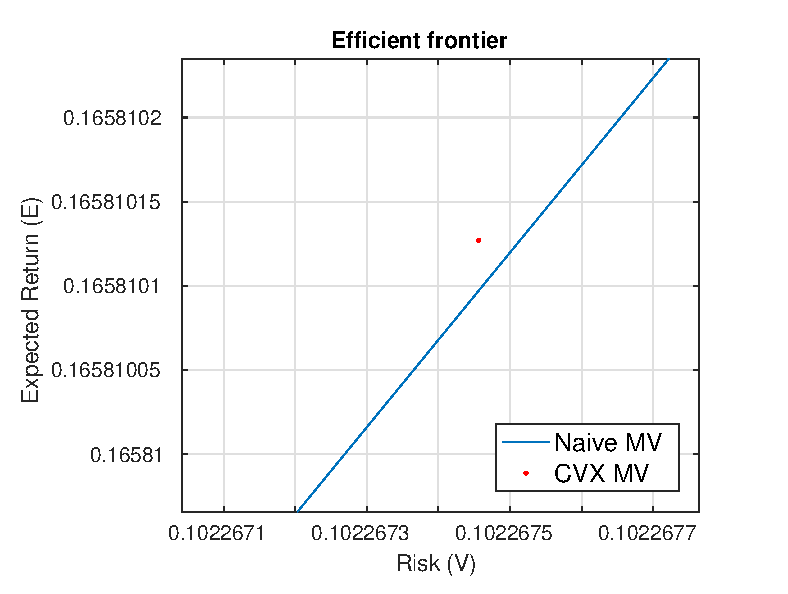
\includegraphics[scale=.5] {q1_d_naive_v_cvx_difference.eps}
       \caption{Difference}
        \label{fig:q1-d-naive-v-cvx-difference}
    \end{subfigure}
    \caption{NaiveMV vs Using CVX}\label{fig:naive_v_cvx}
\end{figure}

The results are extremely similar, since differences only show up in $10^{-7}$ scale. However, the
CVX tool was noticeably slower.

\end{document}



















